\chapter{Réalisation}
	
\section*{Introduction}
\addcontentsline{toc}{section}{Introduction }
    Le quatrième chapitre se consacre à la mise en œuvre concrète du projet. Nous explorons les choix techniques que nous avons adoptés et détaillons le travail effectué pour donner vie à notre solution. De plus, nous parcourons notre workflow en cinq étapes, de l'extraction à la visualisation des données.

\section{Choix technologiques}
\par  Dans cette partie, nous explorerons les décisions stratégiques que nous avons prises concernant les technologies et les outils que nous avons choisis pour la réalisation de notre solution.     
   \begin{itemize}
    \item \textbf{Talend : }
       \par Talend est un outil d'intégration de données open source qui facilite l'extraction, la transformation et le chargement (ETL) des données\cite{talend},Son logo est représenté par la figure \textbf{\ref{fig:talend}}. Il a été utilisé pour gérer le flux de données, les transformations et l'intégration des données dans la base de données. 
          %code image
        \begin{figure}[H]
        \centering
        
\includegraphics[width = 4cm , height=4cm]{img/techno/Talend.png}
        \caption{Logo du Talend\cite{talend}}
        \label{fig:talend}
        \end{figure}
        %fin
    \item \textbf{PostgreSQL : }
    
       \par PostgreSQL est un SGBDR open source \cite{pq}, Son logo est représenté par la figure \textbf{\ref{fig:post}}. Il a été choisi pour stocker et gérer les données collectées dans le projet.
                 %code image
        \begin{figure}[H]
        \centering
        
\includegraphics[width = 4cm , height=4cm]{img/techno/postgresql.png}
        \caption{Logo du PostgreSQL\cite{pg}}
        \label{fig:post}
        \end{figure}
        %fin

    \item \textbf{Streamlit : }
     
       \par Streamlit est un framework Python qui facilite la création d'applications web interactives pour la visualisation de données\cite{streamlit}. Il a été choisi pour concevoir des tableaux de bord interactifs permettant de visualiser les résultats de l'analyse de données de manière conviviale. Son logo est représenté par la figure \textbf{\ref{fig:streamlit}}.
                %code image
        \begin{figure}[H]
        \centering
        
\includegraphics[width = 4cm , height=4cm]{img/techno/streamlit.png}
        \caption{Logo du Streamlit\cite{streamlit}}
        \label{fig:streamlit}
        \end{figure}
        %fin
    \item \textbf{Jira REST API : }
       \par Jira REST API était nécessaire pour extraire des données de Jira. Cela a automatisé la collecte de données, assuré la cohérence et amélioré l'efficacité de l'analyse\cite{JiraRestAPI}. Son logo est représenté par la figure \textbf{\ref{fig:jira}}.
                     %code image
        \begin{figure}[H]
        \centering
        
\includegraphics[width = 4cm , height=4cm]{img/techno/jira.png}
        \caption{Logo du Jira \cite{JiraRestAPI}}
        \label{fig:jira}
        \end{figure}
        %fin
    \item \textbf{Gitlab REST API : }

       \par l'API Gitlab REST a été utilisée pour extraire des données du système de gestion de versions Gitlab. Elle a permis d'automatiser la collecte de données liées au code source, aux commits et aux mesures de performance de l'équipe, renforçant ainsi l'efficacité de l'analyse\cite{GitlabRestAPI}. Son logo est représenté par la figure \textbf{\ref{fig:gitlab}}.
                     %code image
        \begin{figure}[H]
        \centering
        
\includegraphics[width = 4cm , height=4cm]{img/techno/gitlab.png}
        \caption{Logo du Gitlab \cite{GitlabRestAPI}}
        \label{fig:gitlab}
        \end{figure}
        %fin
    \item \textbf{SonarQube REST API : }
       
       \par SonarQube est un outil d'analyse statique du code qui identifie et corrige les problèmes de qualité du code \cite{SonarQube}, son logo est représenté par la figure \textbf{\ref{fig:sonar}}. Son API a permis d'intégrer l'analyse de la qualité du code dans le processus, renforçant ainsi la surveillance et l'amélioration continues.
                   %code image
        \begin{figure}[H]
        \centering
        
\includegraphics[width = 4cm , height=2.5cm]{img/techno/sonarqube.png}
        \caption{Logo du sonarQube \cite{SonarQube}}
        \label{fig:sonar}
        \end{figure}
        %fin
    \item \textbf{Numpy: }
        
       \par NumPy est une bibliothèque essentielle pour le calcul numérique en Python \cite{numpy}, son logo est représenté par la figure \textbf{\ref{fig:numpy}}. Elle offre des structures de données et des fonctions pour effectuer des opérations mathématiques et statistiques sur des tableaux, ce qui est précieux pour la manipulation et l'analyse des données dans le projet.
             %code image
        \begin{figure}[H]
        \centering
        
\includegraphics[width = 4cm , height=2.5cm]{img/techno/numpy.png}
        \caption{Logo du Numpy\cite{numpy}}
        \label{fig:numpy}
        \end{figure}
        %fin
    \item \textbf{Pandas: }
       \par Pandas est une bibliothèque de manipulation de données  Python qui fournit des structures de données flexibles pour l'analyse des données\cite{pandas} , son logo est représenté par la figure \textbf{\ref{fig:pandas}}. Elle facilite l'importation, la manipulation et l'analyse des données provenant de diverses sources, ce qui en fait un choix idéal pour votre projet.
             %code image
        \begin{figure}[H]
        \centering
        
\includegraphics[width = 4cm , height=2.5cm]{img/techno/pandas.png}
        \caption{Logo du Pandas\cite{pandas}}
        \label{fig:pandas}
        \end{figure}
        %fin
       
   \end{itemize}

\section{Exécution du workflow }
    \par Gérer efficacement le flux de travail est d'une importance capitale pour notre projet, car il guide chacune des étapes du processus, depuis l'extraction initiale des données jusqu'à leur transformation, leur stockage intérimaire et leur analyse.
    \par Dans cette section, nous plongerons en profondeur dans chacune des étapes du flux de travail, exposant les méthodes, les outils et les solutions pour relever les défis qui se présentent. Notre objectif est de présenter un processus fluide et cohérent, démontrant comment chaque phase contribue à la qualité des données et à l'évaluation de la performance de l'équipe Avaxia.
        \subsection{Exctraction des données }
    
        \par Dans la phase initiale de notre projet, nous avons commencé par extraire des données à partir de plusieurs sources essentielles, dont Jira et GitHub. Cette extraction de données s'est effectuée en utilisant des REST API dédiées à chaque plateforme, ce qui a permis une collecte systématique et automatisée des informations et nous avons procédé comme suit:
        \begin{itemize}
            \item \par\textbf{ Gestion de la sécurité des données:} la sécurité des données a constitué une préoccupation majeure durant cette étape initiale. Nous avons mis en place des mesures de sécurité rigoureuses pour préserver l'intégrité des informations sensibles. Cela englobait des processus d'authentification et d'autorisation d'accès aux API, ainsi que des protocoles de stockage des données extraites garantissant leur confidentialité.
             \item \par\textbf{Défi de la diversité des sources de données: }un défi significatif auquel nous avons fait face était la disparité des formats de données entre les différentes plateformes. Chacune d'entre elles présentait sa propre structure et ses schémas de données distincts. Pour s'assurer de la cohérence et de la comparabilité des données extraites, nous avons dû les normaliser. Cela impliquait de les convertir dans un format standardisé et compatible avec notre système de gestion de base de données.
        \end{itemize}
        \par À la fin de cette étape, nous avons disposé d'une quantité considérable de données brutes provenant de diverses sources. Ces données représentaient la base sur laquelle nous allions construire nos analyses ultérieures.


        \begin{figure}[H]
            \centering
            %\subfloat{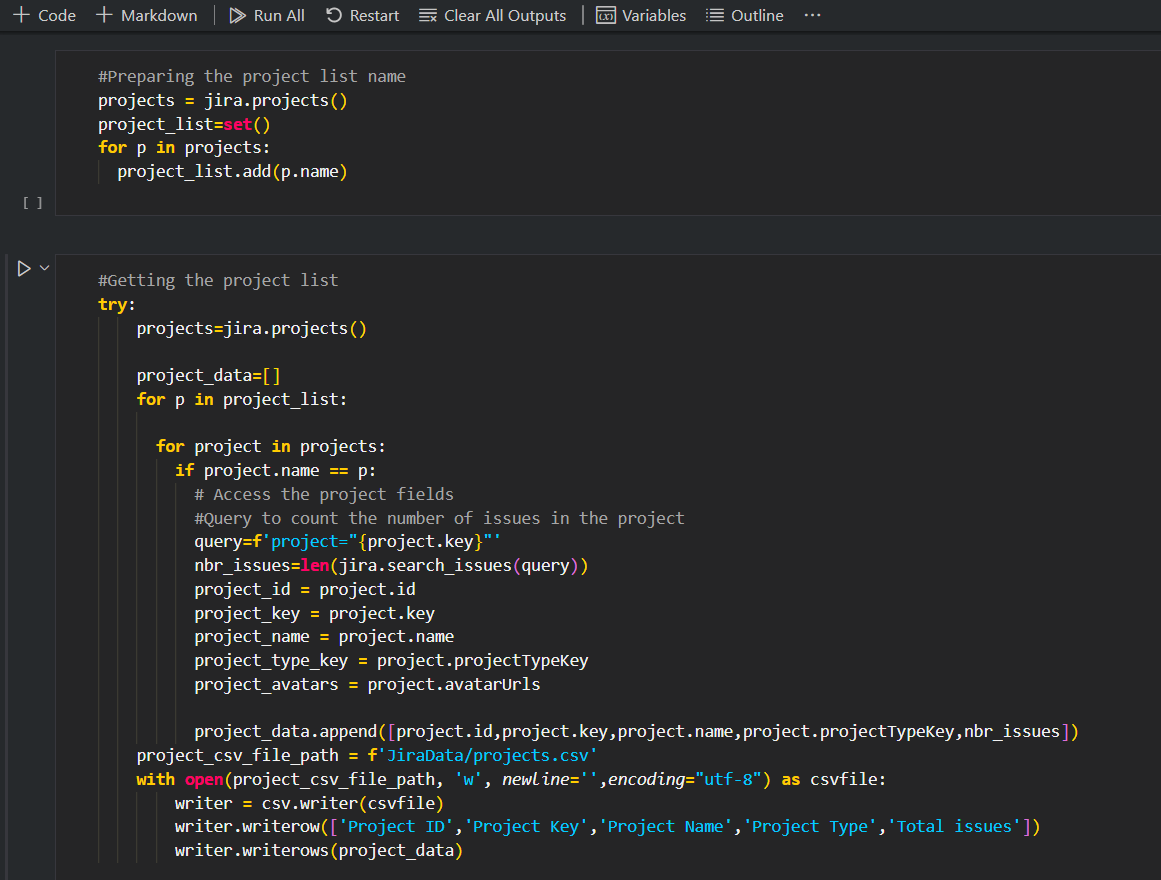
\includegraphics[width=1\linewidth, height=9cm]{img/captures/2.png}} \hspace{0.1cm}
            \caption{Exemple d'extraction des données "Project Extractions"}
            \label{fig:extract}

        \end{figure}

        \par Les figures qui suit projette des exemples des données extraites:
    \begin{itemize}
            
       \item  Les données représentées dans la figure \textbf{\ref{fig:projects}} suivante illustres une partie de la liste des projets de Avaxia:
        \begin{figure}[H]
             \begin{minipage}{1\linewidth}
                \centering
               % \subfloat{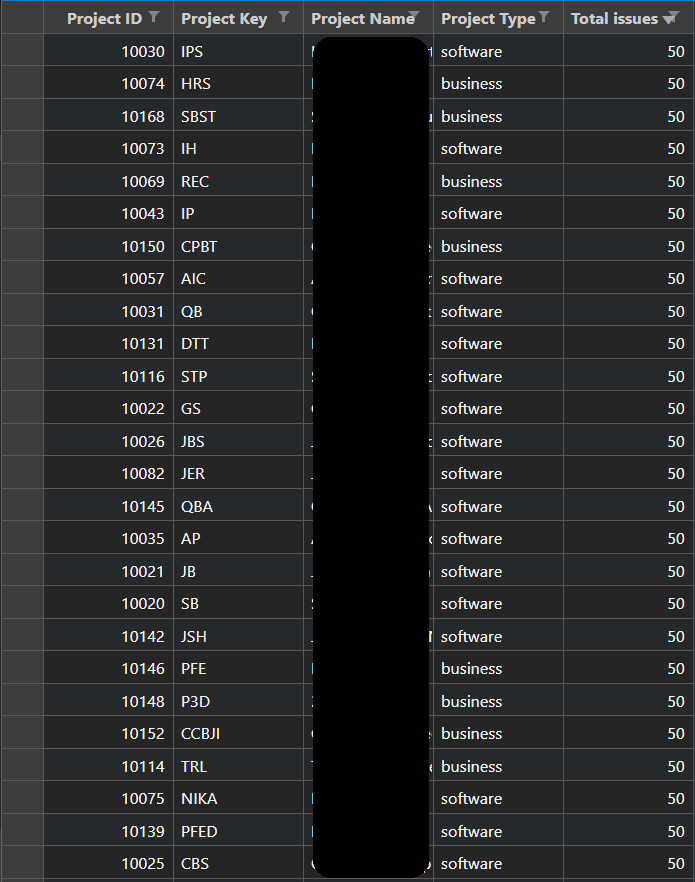
\includegraphics[width=7.5cm , height=8.5cm]{img/captures/projects.png}}\hspace{0.5cm} 
                %\subfloat{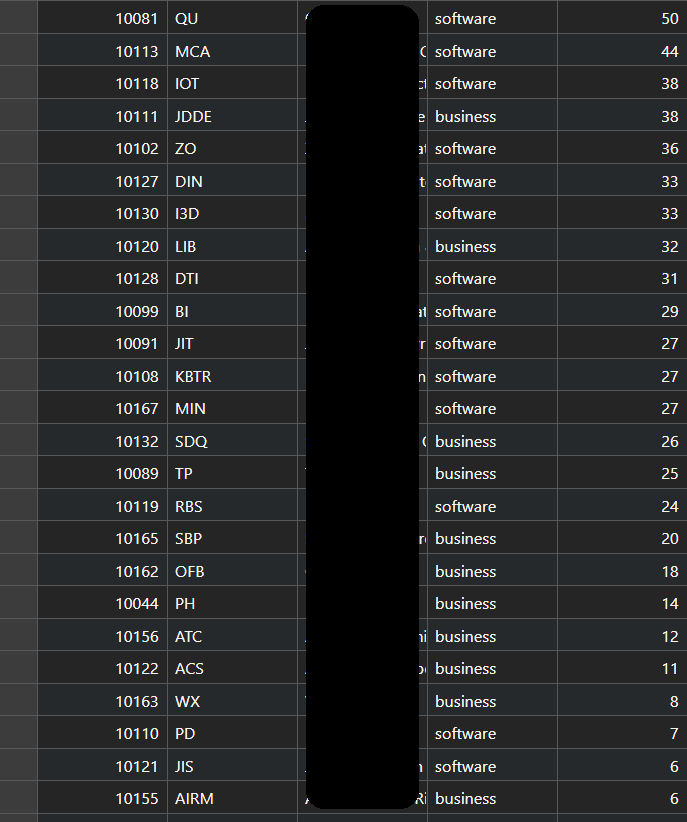
\includegraphics[width=7.5cm , height=8.5cm]{img/captures/projects2.png}}
                \caption{Extrait des données collectés des projects}
                             \label{fig:projects}

            \end{minipage}\hfill 
            \begin{minipage}{1\linewidth}
                \centering
 
            \end{minipage}
             \label{fig:login}
        \end{figure}
        \newpage
        \item  Les données représentées dans la figure \textbf{\ref{fig:boards}} suivante illustres une partie des tableaux Jira(boards) dont les projets sont affectés.
        \begin{figure}[H]
            
             \begin{minipage}{1\linewidth}
                \centering
                %\subfloat{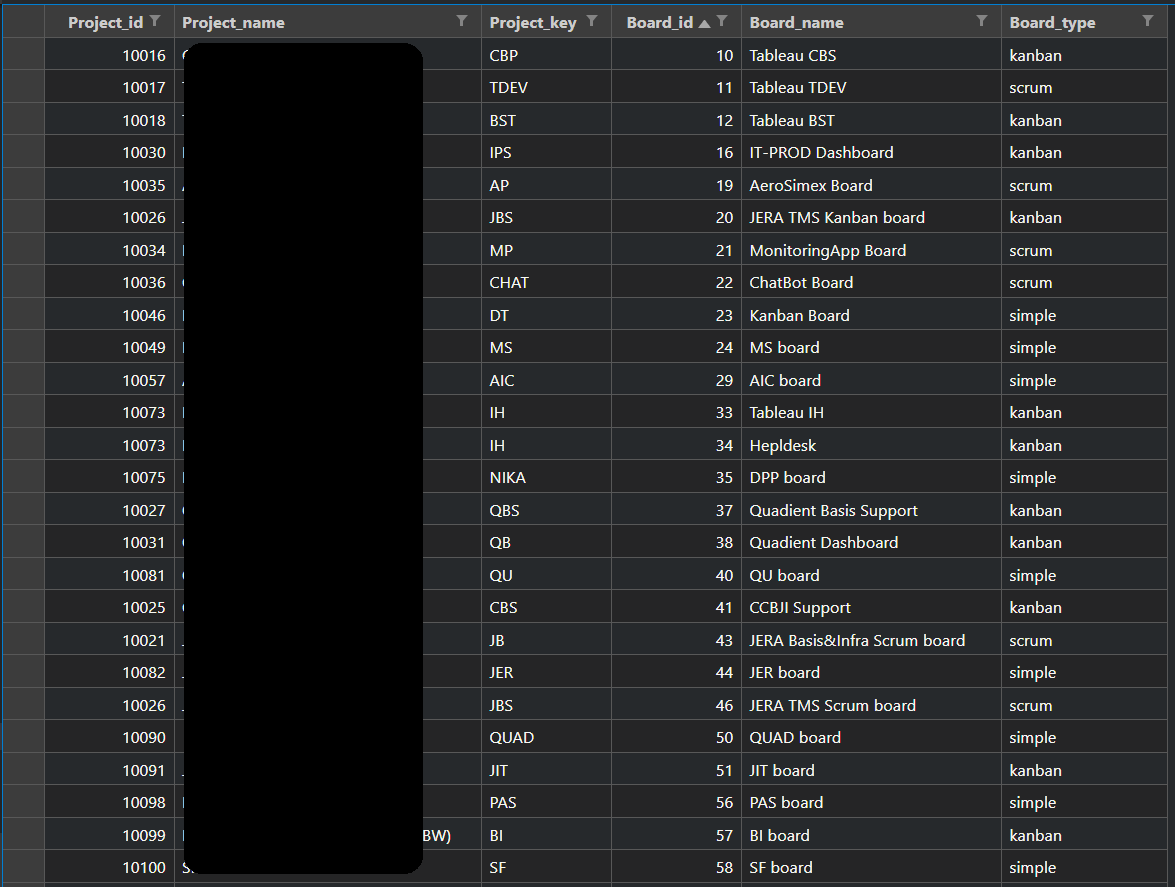
\includegraphics[width=1\linewidth, height=9cm]{img/captures/boards.png}}
                \caption{Extrait des données collectées des tableaux jira}
                    \label{fig:boards}

            \end{minipage}\hfill 
            \begin{minipage}{1\linewidth}
                \centering
                
            \end{minipage}
             \label{fig:login}
        \end{figure}
        \item  Les données représentées dans la figure \textbf{\ref{fig:users}} suivante illustres une partie des la liste des utilisateurs(collaborateurs).
        \begin{figure}[H]
            
             \begin{minipage}{1\linewidth}
                \centering
                %\subfloat{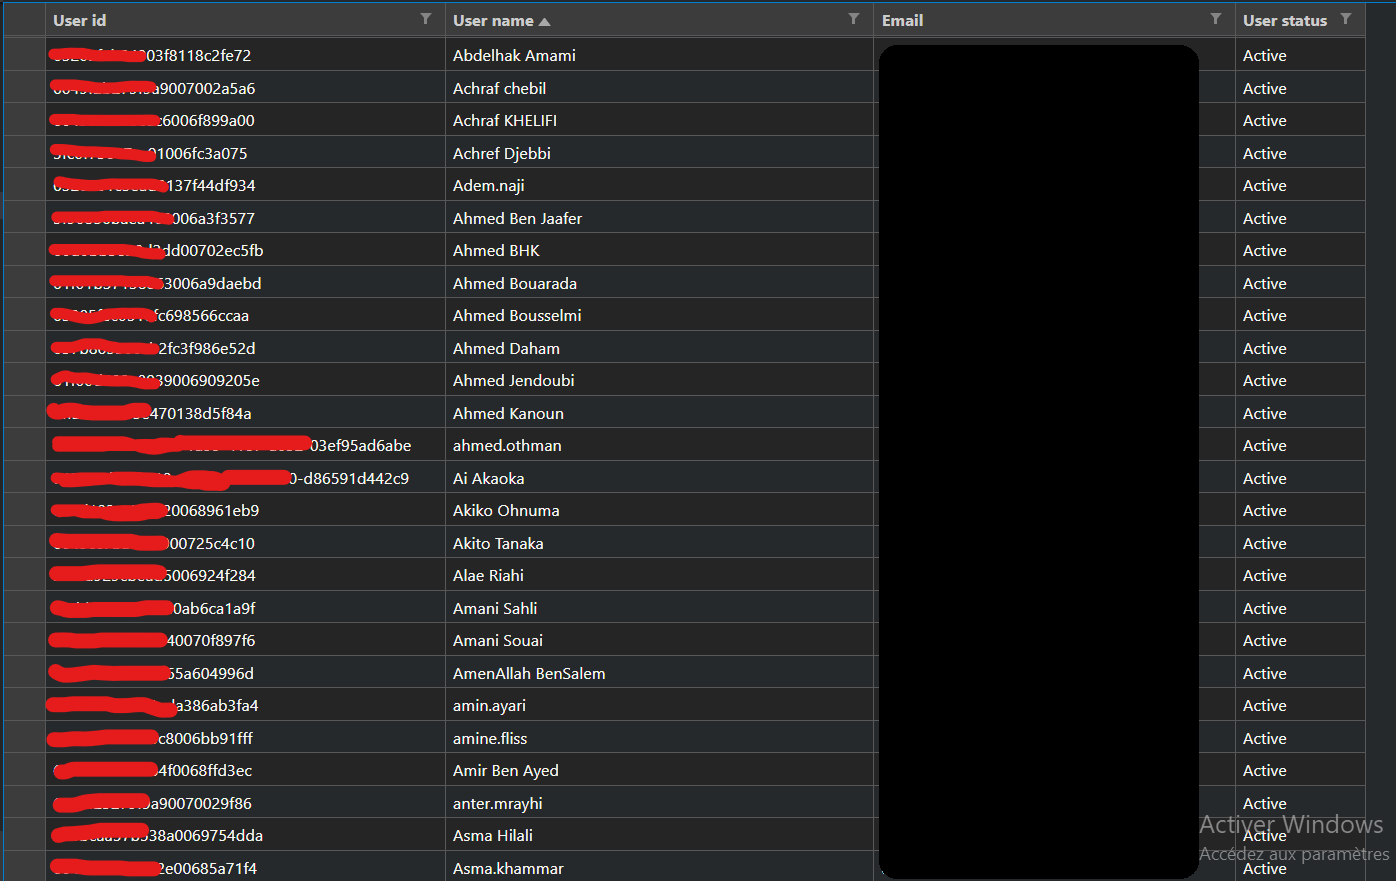
\includegraphics[width=1\linewidth, height=9cm]{img/captures/users.png}}
                \caption{Extrait des données collectées des utilisateurs}
                \label{fig:users}

            \end{minipage}\hfill 
            \begin{minipage}{1\linewidth}
                \centering
                
            \end{minipage}
             \label{fig:login}
        \end{figure}
        \item  Les données représentées dans la figure \textbf{\ref{fig:issues}} suivante une partie des la liste des tickets jira(issues).
        \begin{figure}[H]
            
             \begin{minipage}{1\linewidth}
                \centering
                %\subfloat{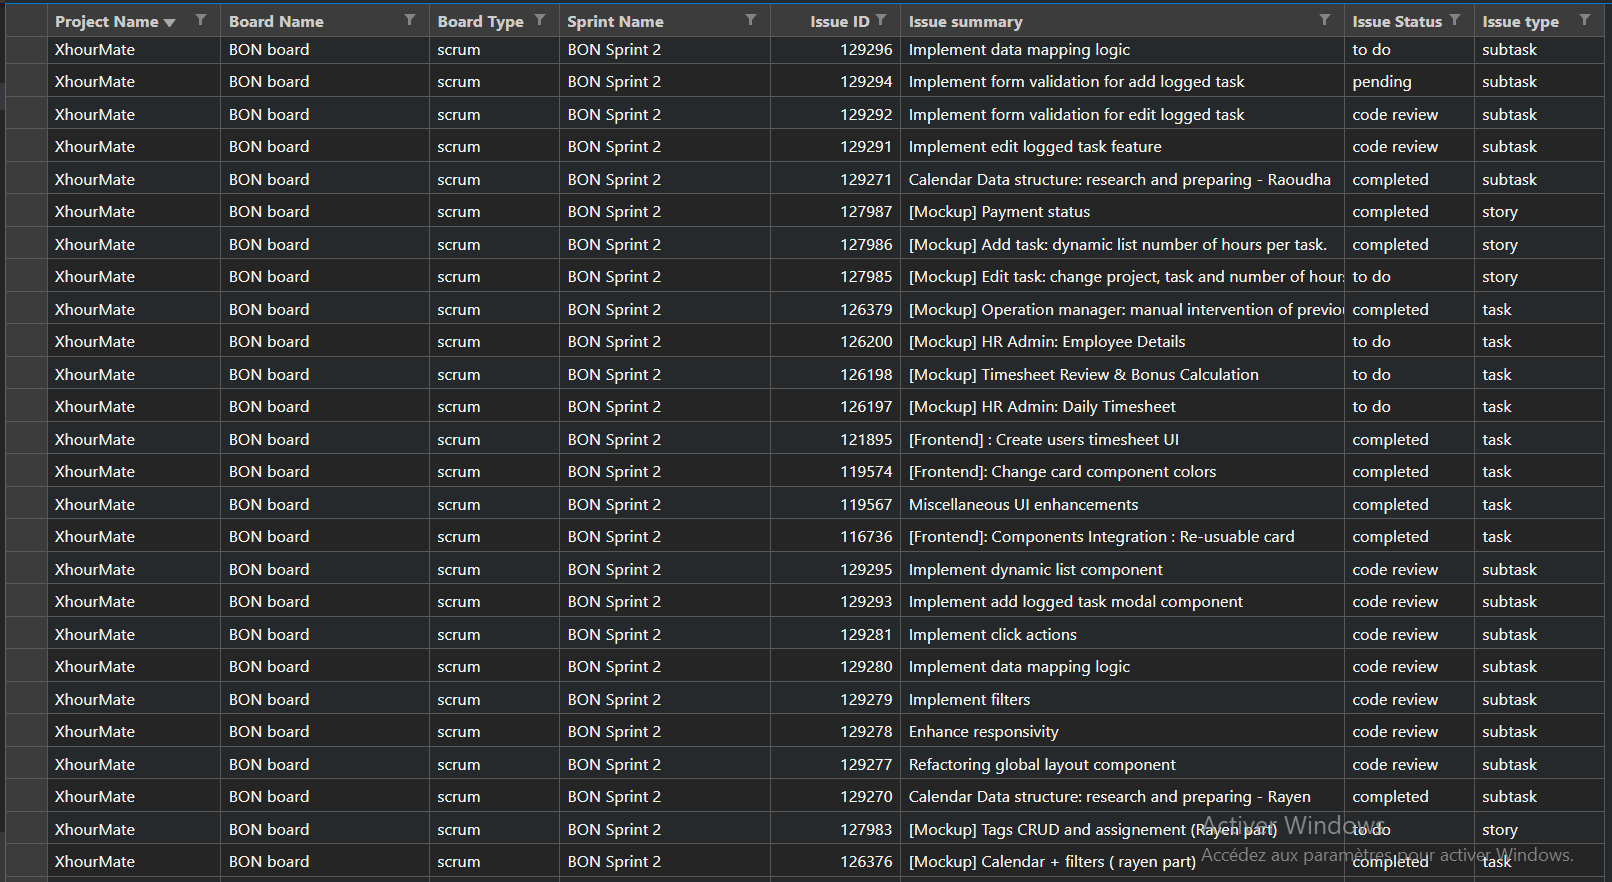
\includegraphics[width=1\linewidth , height=10cm]{img/captures/issues.png}}
                \caption{Extrait des données collectées des tickets}
                \label{fig:issues}

            \end{minipage}\hfill 
            \begin{minipage}{1\linewidth}
                \centering
                
            \end{minipage}
             \label{fig:login}
        \end{figure}
    \end{itemize}
        \par L'extraction des données constitue une phase cruciale, car elle fournit la matière première fondamentale pour notre projet. Ces données brutes forment la base de notre analyse ultérieure. Il est toutefois important de noter que cette étape ne représente que le point de départ de notre workflow. Les données extraites nécessitent encore une préparation, un nettoyage et une analyse approfondie pour en extraire des informations significatives, un aspect que nous explorerons en détail dans les prochaines phases.
        \subsection{Transformation des données}
        \par Au cours de cette étape cruciale, nous avons traité les données brutes extraites de diverses sources pour les préparer à l'analyse ultérieure. Cette phase de transformation était essentielle pour s'assurer que les données étaient cohérentes, complètes et prêtes à être exploitées. Voici comment nous avons procédé avec plus de détails:
        \begin{itemize}
            \item \textbf{Exploration des données:} nous avons commencé par explorer les données brutes pour comprendre leur structure et leur qualité. Cela incluait l'examen des différents formats, des types de données, des valeurs manquantes, des doublons et d'autres caractéristiques.
        
            \item \textbf{Nettoyage des données:} pour garantir la qualité des données, nous avons entrepris un processus de nettoyage rigoureux. Cela impliquait la correction des valeurs incorrectes, la suppression des doublons, le comblement des valeurs manquantes, et la normalisation des données lorsque cela était nécessaire.
            \item \textbf{Transformation et structuration:} Les données brutes étant souvent non structurées, nous les avons transformées en une forme structurée. Cela comprenait la création de schémas de données cohérents et l'organisation des informations en fonction de nos besoins d'analyse.
            \item \textbf{Filtrage des données:} certaines données étaient excessivement volumineuses ou non pertinentes pour notre objectif d'analyse. Nous avons donc appliqué des filtres pour ne conserver que les données pertinentes et significatives.

            \item \textbf{Enrichissement des données:} dans certains cas, nous avons enrichi les données en ajoutant des informations supplémentaires à partir d'autres sources. Cela visait à renforcer la qualité et la pertinence des données.
            \item \textbf{Stockage intermédiaire:} les données transformées ont été stockées de manière sécurisée dans des fichiers CSV, prêtes à être utilisées pour l'analyse ultérieure.

            \par les figures \textbf{\ref{fig:avant}} et \textbf{\ref{fig:apres}} suivantes illustre des exemples des données brutes et redondantes avant  et après la phase de transformation des données qui sont stocker dans des fichiers CSV.
            
            \begin{figure}[H]
                \centering
                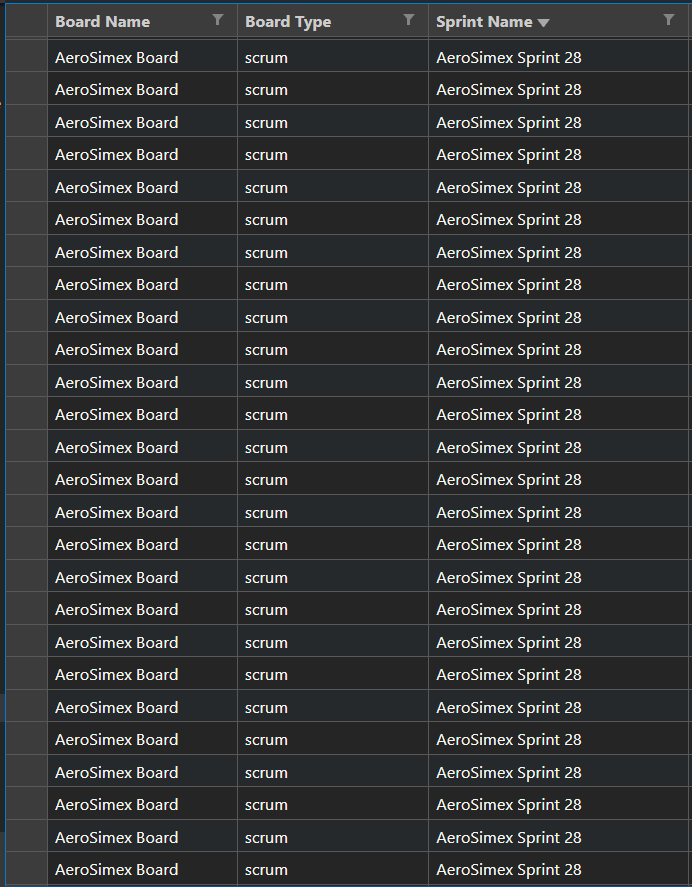
\includegraphics[width=1\linewidth, height=9cm]{img/captures/sprints.png}
                \caption{Exemple des données brutes et erronées avec doublements des valeurs}
                \label{fig:avant}
            \end{figure}
            \begin{figure}[H]
                    \centering
                    \includegraphics[width=1\linewidth, height=9cm]{img//captures/sprintsafter.png}
                    \caption{Exemple des données des sprints après la phase de transformation}
                \label{fig:apres}

            \end{figure}
        \end{itemize}
        \par L'étape de transformation des données était une étape cruciale pour garantir que les informations extraites étaient fiables et prêtes pour l'analyse. Elle exigeait une attention méticuleuse aux détails, un processus systématique de nettoyage et de structuration, et une compréhension approfondie des spécificités des données de votre projet.
        
        \subsection{Chargement des Données}
        \par Après avoir extrait et transformé les données, la prochaine phase de notre workflow était le chargement des données. Au cours de cette étape, nous avons acheminé les données nettoyées et transformées vers notre système de gestion de base de données, en l'occurrence PostgreSQL. Voici un aperçu détaillé de cette étape cruciale :
        \begin{itemize}
            \item \textbf{Benchmarking et choix de PostgreSQl}: avant de prendre notre décision, nous avons effectué un benchmarking minutieux en comparant plusieurs systèmes de gestion de bases de données. PostgreSQL a émergé comme le choix optimal en raison de sa flexibilité, de ses performances exceptionnelles et de sa capacité à gérer des charges de travail complexes. Cette étape a jeté les bases pour une intégration réussie.
            \par la figure \textbf{\ref{fig:bench}} illustre le benchmarking effectué par le code ci-dessous: 
            \begin{figure}[H]
                \centering
                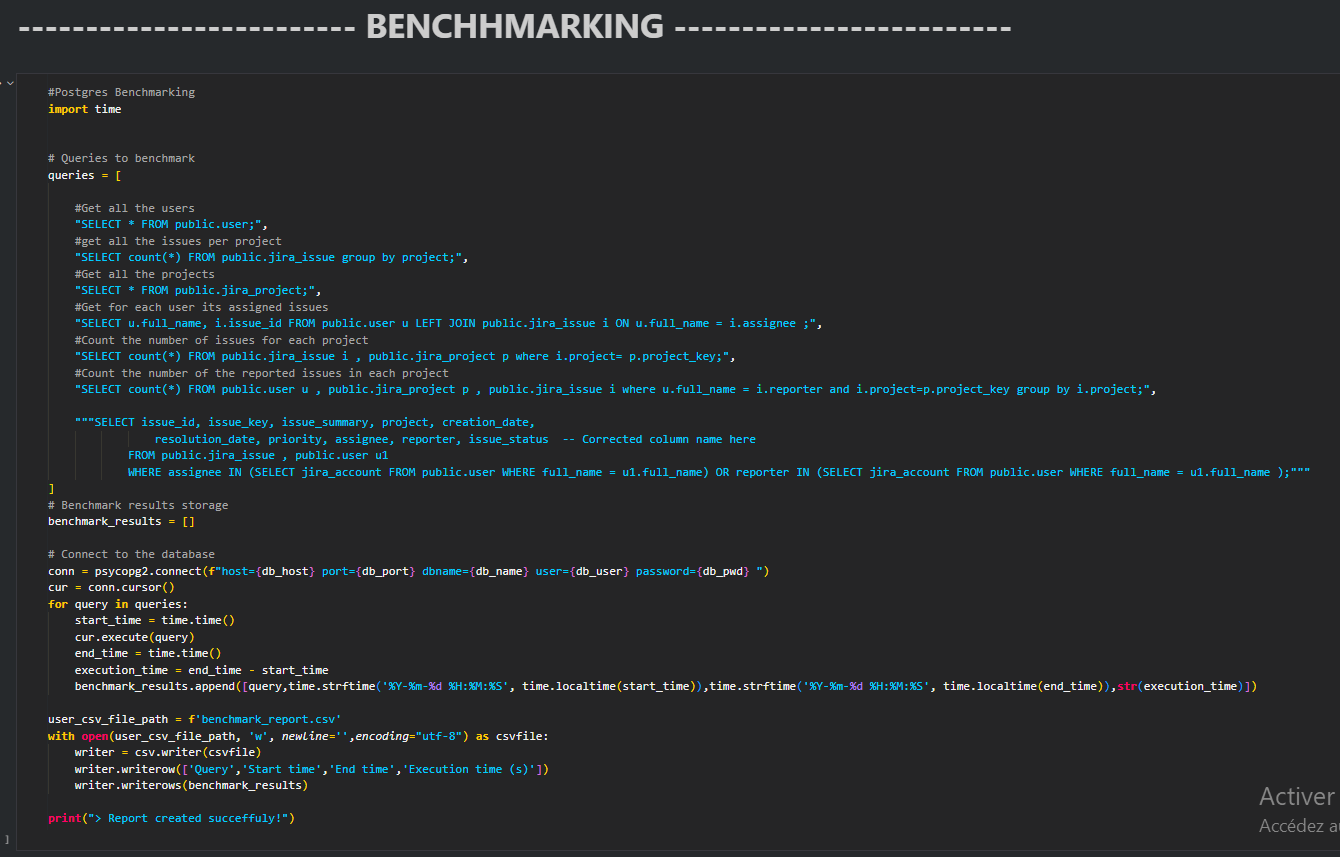
\includegraphics[width=1\linewidth, height=8cm]{img//captures/benchmarking.png}
                \caption{Code de benchmarking d'une base de donné secondaire}
                \label{fig:bench}
            \end{figure}
            \par la figure \textbf{\ref{fig:report}} suivante donne le rapport de benchmarking qui illustre la perfermance de la base de données postgreSQL en terme d'accés aux données : 
            \begin{figure}[H]
                \centering
                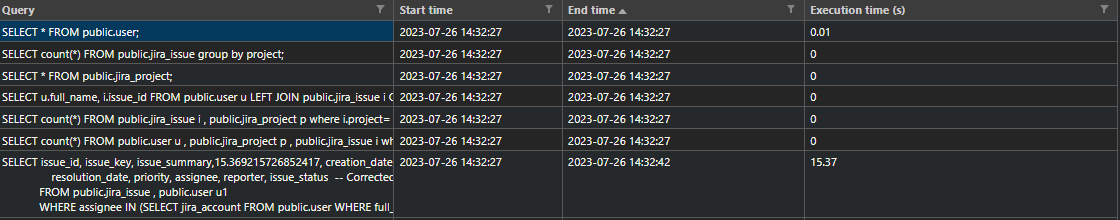
\includegraphics[width=1\linewidth, height=3cm]{report_bench.png}
                \caption{Rapport de benchmarking PostgreSQL}
                \label{fig:report}
            \end{figure}
            
            \item \textbf{Intégration avec PostgreSQL}: nous avons créé des flux de données pour transférer les données transformées vers notre base de données PostgreSQL. Cette intégration a permis de stocker de manière centralisée toutes les informations nécessaires à nos analyses.
            \par la figure \textbf{\ref{fig:database}} suivante illustre le dshboard de la base de données sur PgAdmin( qui est l'outil de gestion de base de données PostgreSQL) :
            \begin{figure}[H]
            \centering
            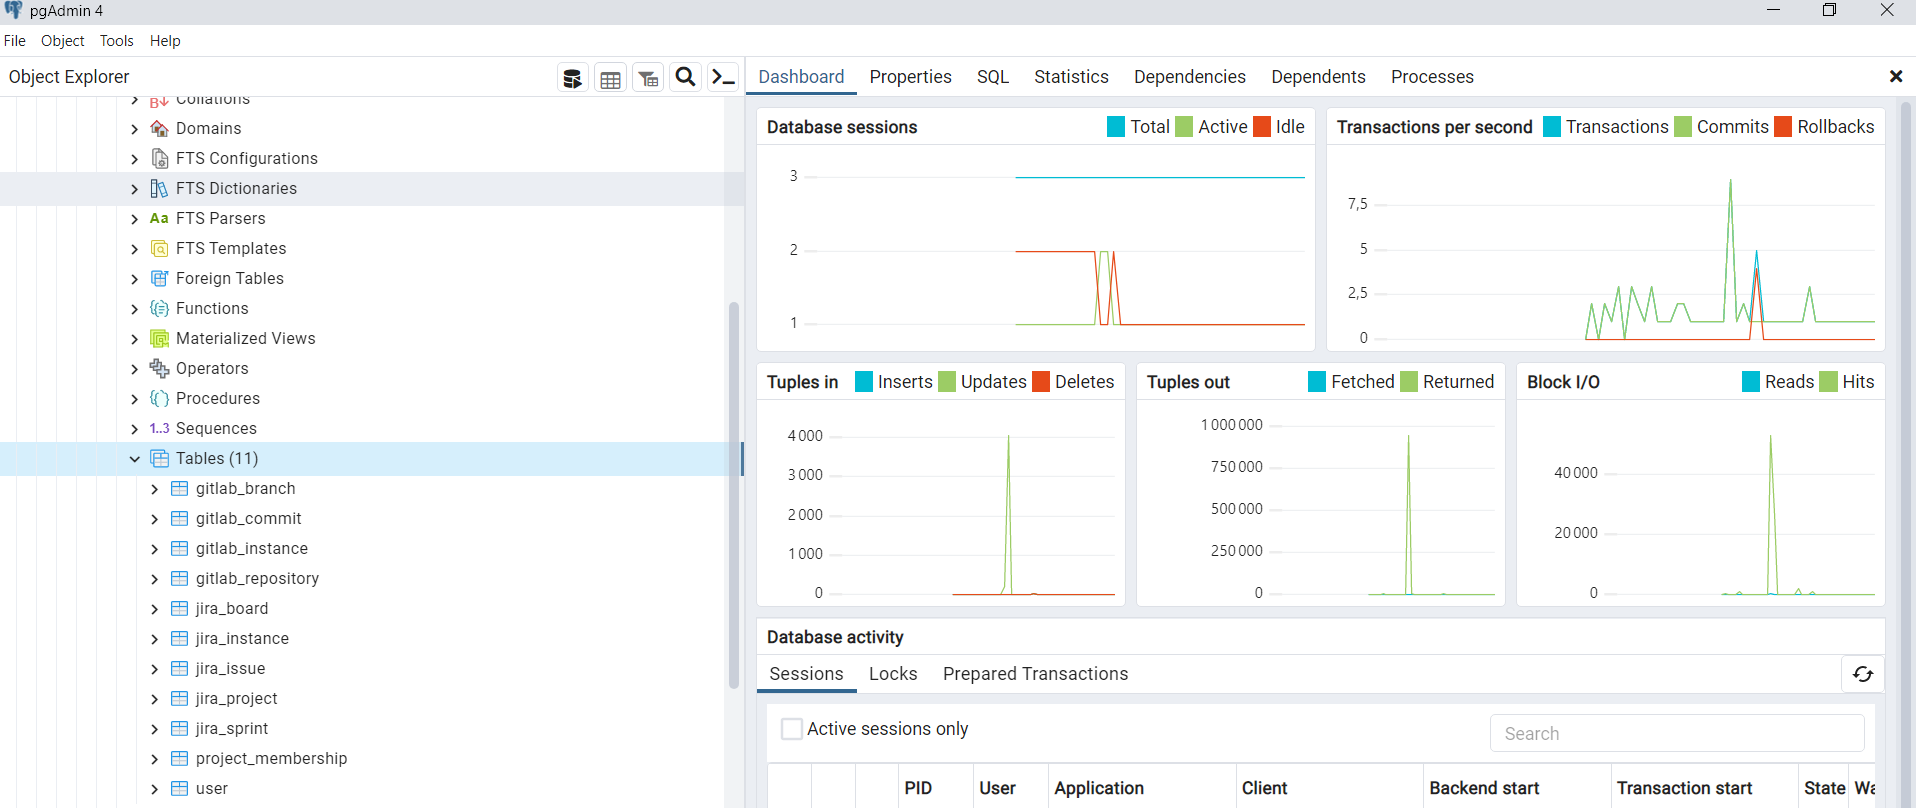
\includegraphics[width=17cm , height=9cm]{img//captures/postgres.png}
            \caption{Enter Caption}
            \label{fig:database}
            \end{figure}
            \item \textbf{Garantie de la cohérence}: lors du chargement des données, il était essentiel de veiller à la cohérence et à l'intégrité des données. Des mécanismes de validation ont été mis en place pour éviter toute altération ou perte de données lors du transfert.
            \item \textbf{Sécurité des données}: la sécurité des données était une priorité constante. Nous avons mis en place des mesures de sécurité pour protéger les données sensibles tout au long de leur trajet vers la base de données.
            \item \textbf{Sauvegarde et récupération}: des procédures de sauvegarde régulières ont été mises en place pour garantir la disponibilité des données en cas de sinistre ou de défaillance du système.
        \end{itemize}
        \par les figures qui suit illustrent des échantillons des données stockées dans les différents tables de la base:
        \par la figure \textbf{\ref{fig:issue_table}} projette une partie des données de la table <<JiraIssues>>
        \begin{figure}[H]
            \centering
            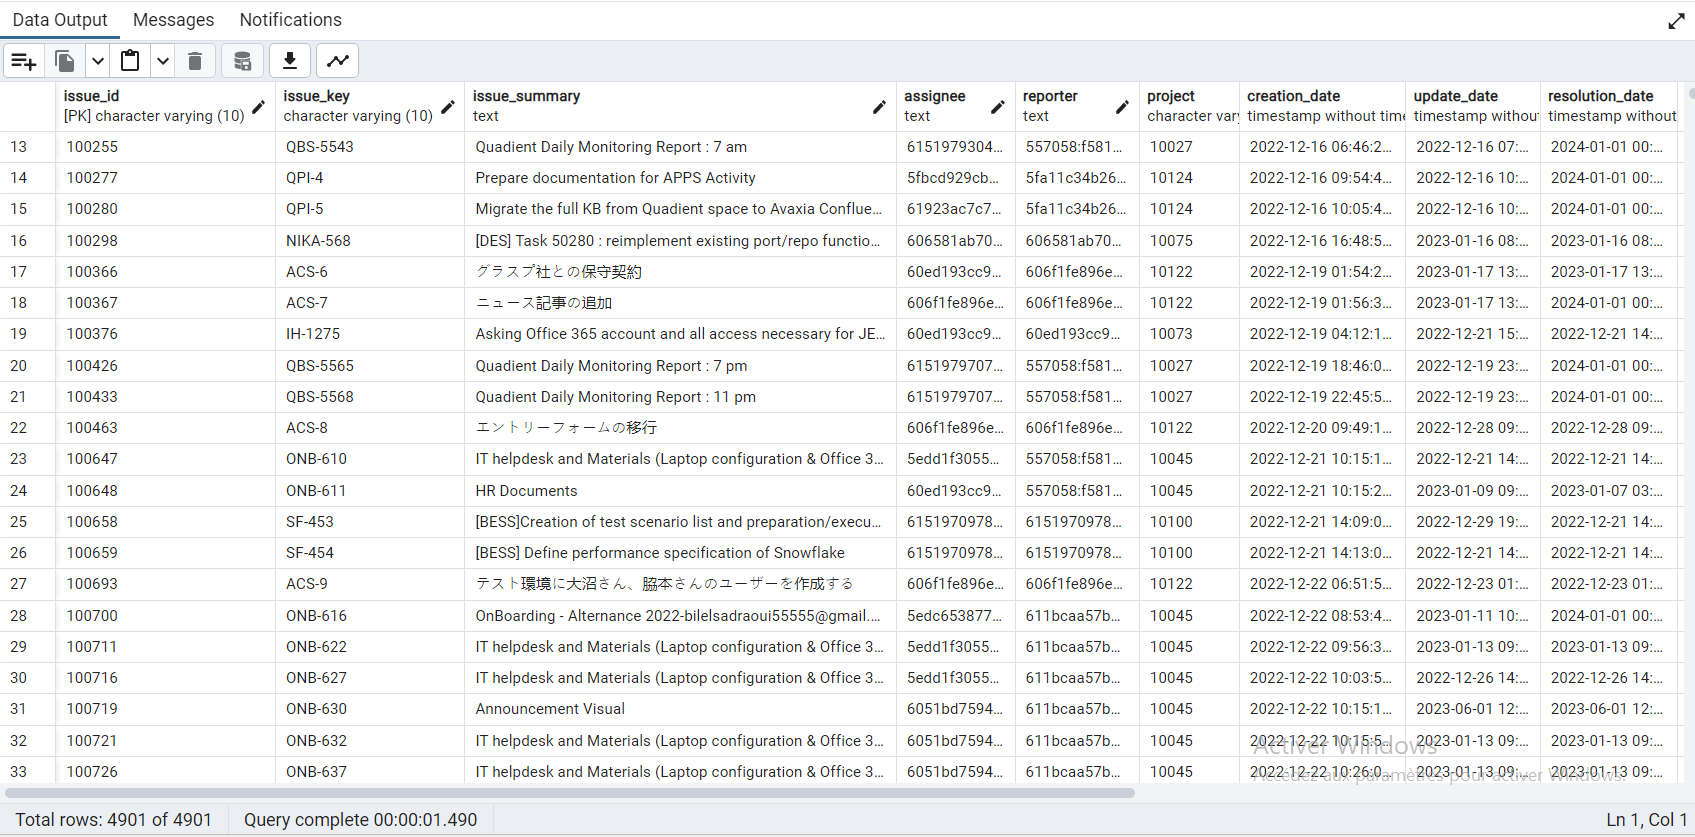
\includegraphics[width=1\linewidth]{img//conception/issues.png}
            \caption{Lignes de la table <<JiraIssues>>}
            \label{fig:issue_table}
        \end{figure}
        
        \par L'étape de chargement des données était fondamentale pour centraliser nos informations dans une base de données prête à être consultée et analysée. Ces données étaient maintenant accessibles de manière efficace, ce qui a constitué la base de notre workflow d'analyse des performances de l'équipe Avaxia.
        \subsection{Analyse des données}
        \par Une fois les données extraites, transformées et chargées dans notre base de données, nous avons progressé vers la phase cruciale de l'analyse des données. L'objectif était de tirer des enseignements concrets à partir des données brutes que nous avions recueillies. Voici comment cette étape s'est déroulée en détail :
        \begin{itemize}
            \item \textbf{Exploration des données:} nous avons initié cette phase par une exploration méticuleuse des données. Notre démarche consistait à visualiser les données sous différentes perspectives, à identifier les tendances et les valeurs aberrantes, et à acquérir une compréhension profonde de la structure des informations disponibles. Cette exploration initiale a fourni des indications cruciales sur la nature des données, orientant ainsi nos futures analyses.
            \par Les figures \textbf{\ref{fig:user_status}} et \textbf{\ref{fig:user_table}} suivantes représentent quelques fonctions utilisées pour l'extraction des corrélations et à identifier les tendances et les valeurs aberrantes:
            \begin{figure}[H]
                \centering
                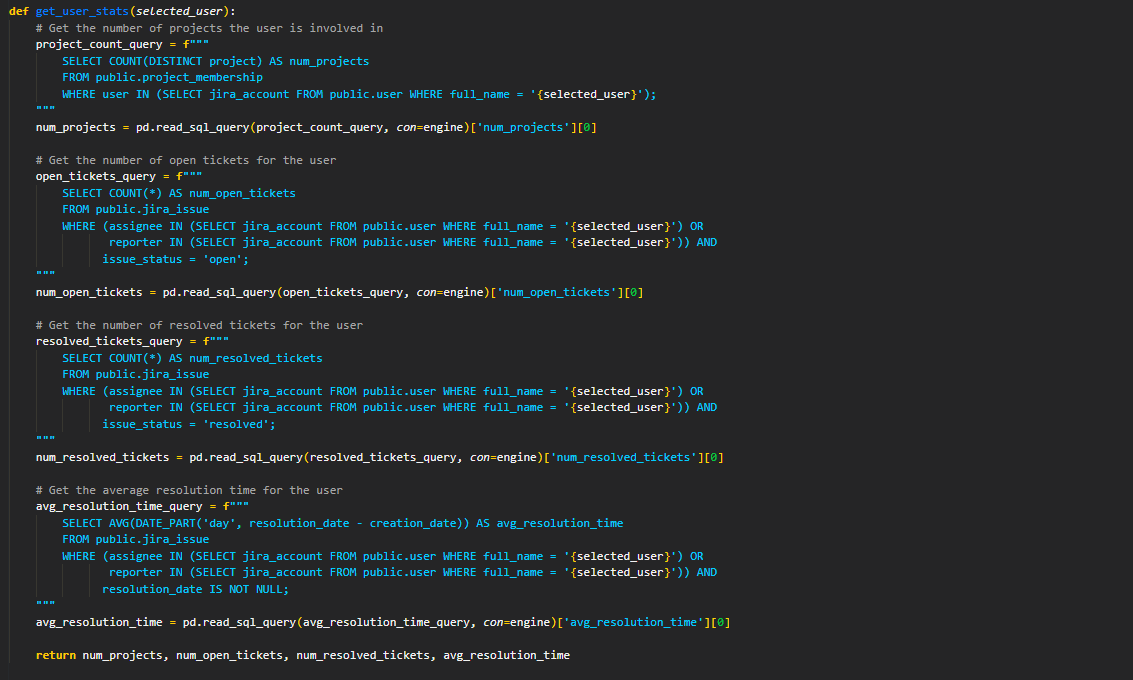
\includegraphics[width=1\linewidth]{img//captures/user_status.png}
                \caption{Un bout de code qui traite les status des utilisateurs selon leurs affectations aux tickets  <<USER>>}
                \label{fig:user_status}
            \end{figure}
            \begin{figure}[H]
                \centering
                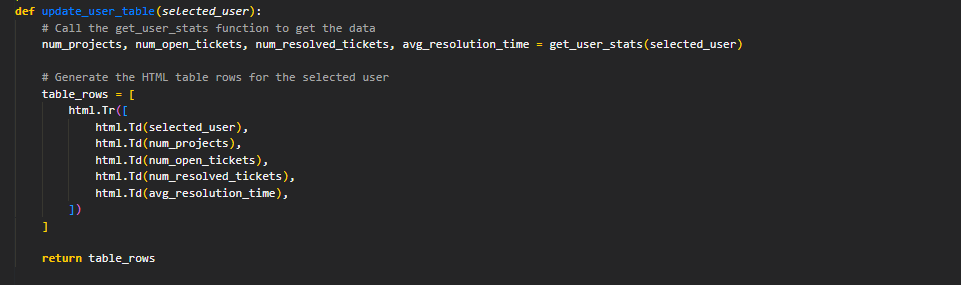
\includegraphics[width=\linewidth]{img/captures/table_users.png}
                \caption{Un bout de code qui traite la table de données <<USER>>}
                \label{fig:user_table}
            \end{figure}
            \item \textbf{Analyse statistique:} une fois que nous avons sondé en profondeur les données, nous avons entrepris des analyses statistiques approfondies. Ces analyses ont fait appel à des techniques de calcul, des méthodes statistiques et des modèles prédictifs pour extraire des informations significatives. Nous avons effectué des calculs de corrélation, des tests statistiques et développé des modèles prédictifs pour évaluer la performance de l'équipe Avaxia.
            \par Grâce à ces modelés développer, nous avons réussi à extraire des corrélations entre les données de notre base qui ont été représenté ultérieurement par des graphes de corrélation.
            \par La figure \textbf{\ref{fig:cycle}}représente le graphe de corrélation entre le temps des resolution des tickets et le nombres des tickets affectés à chaque collaborateur:
            \begin{figure}[H]
                \centering
                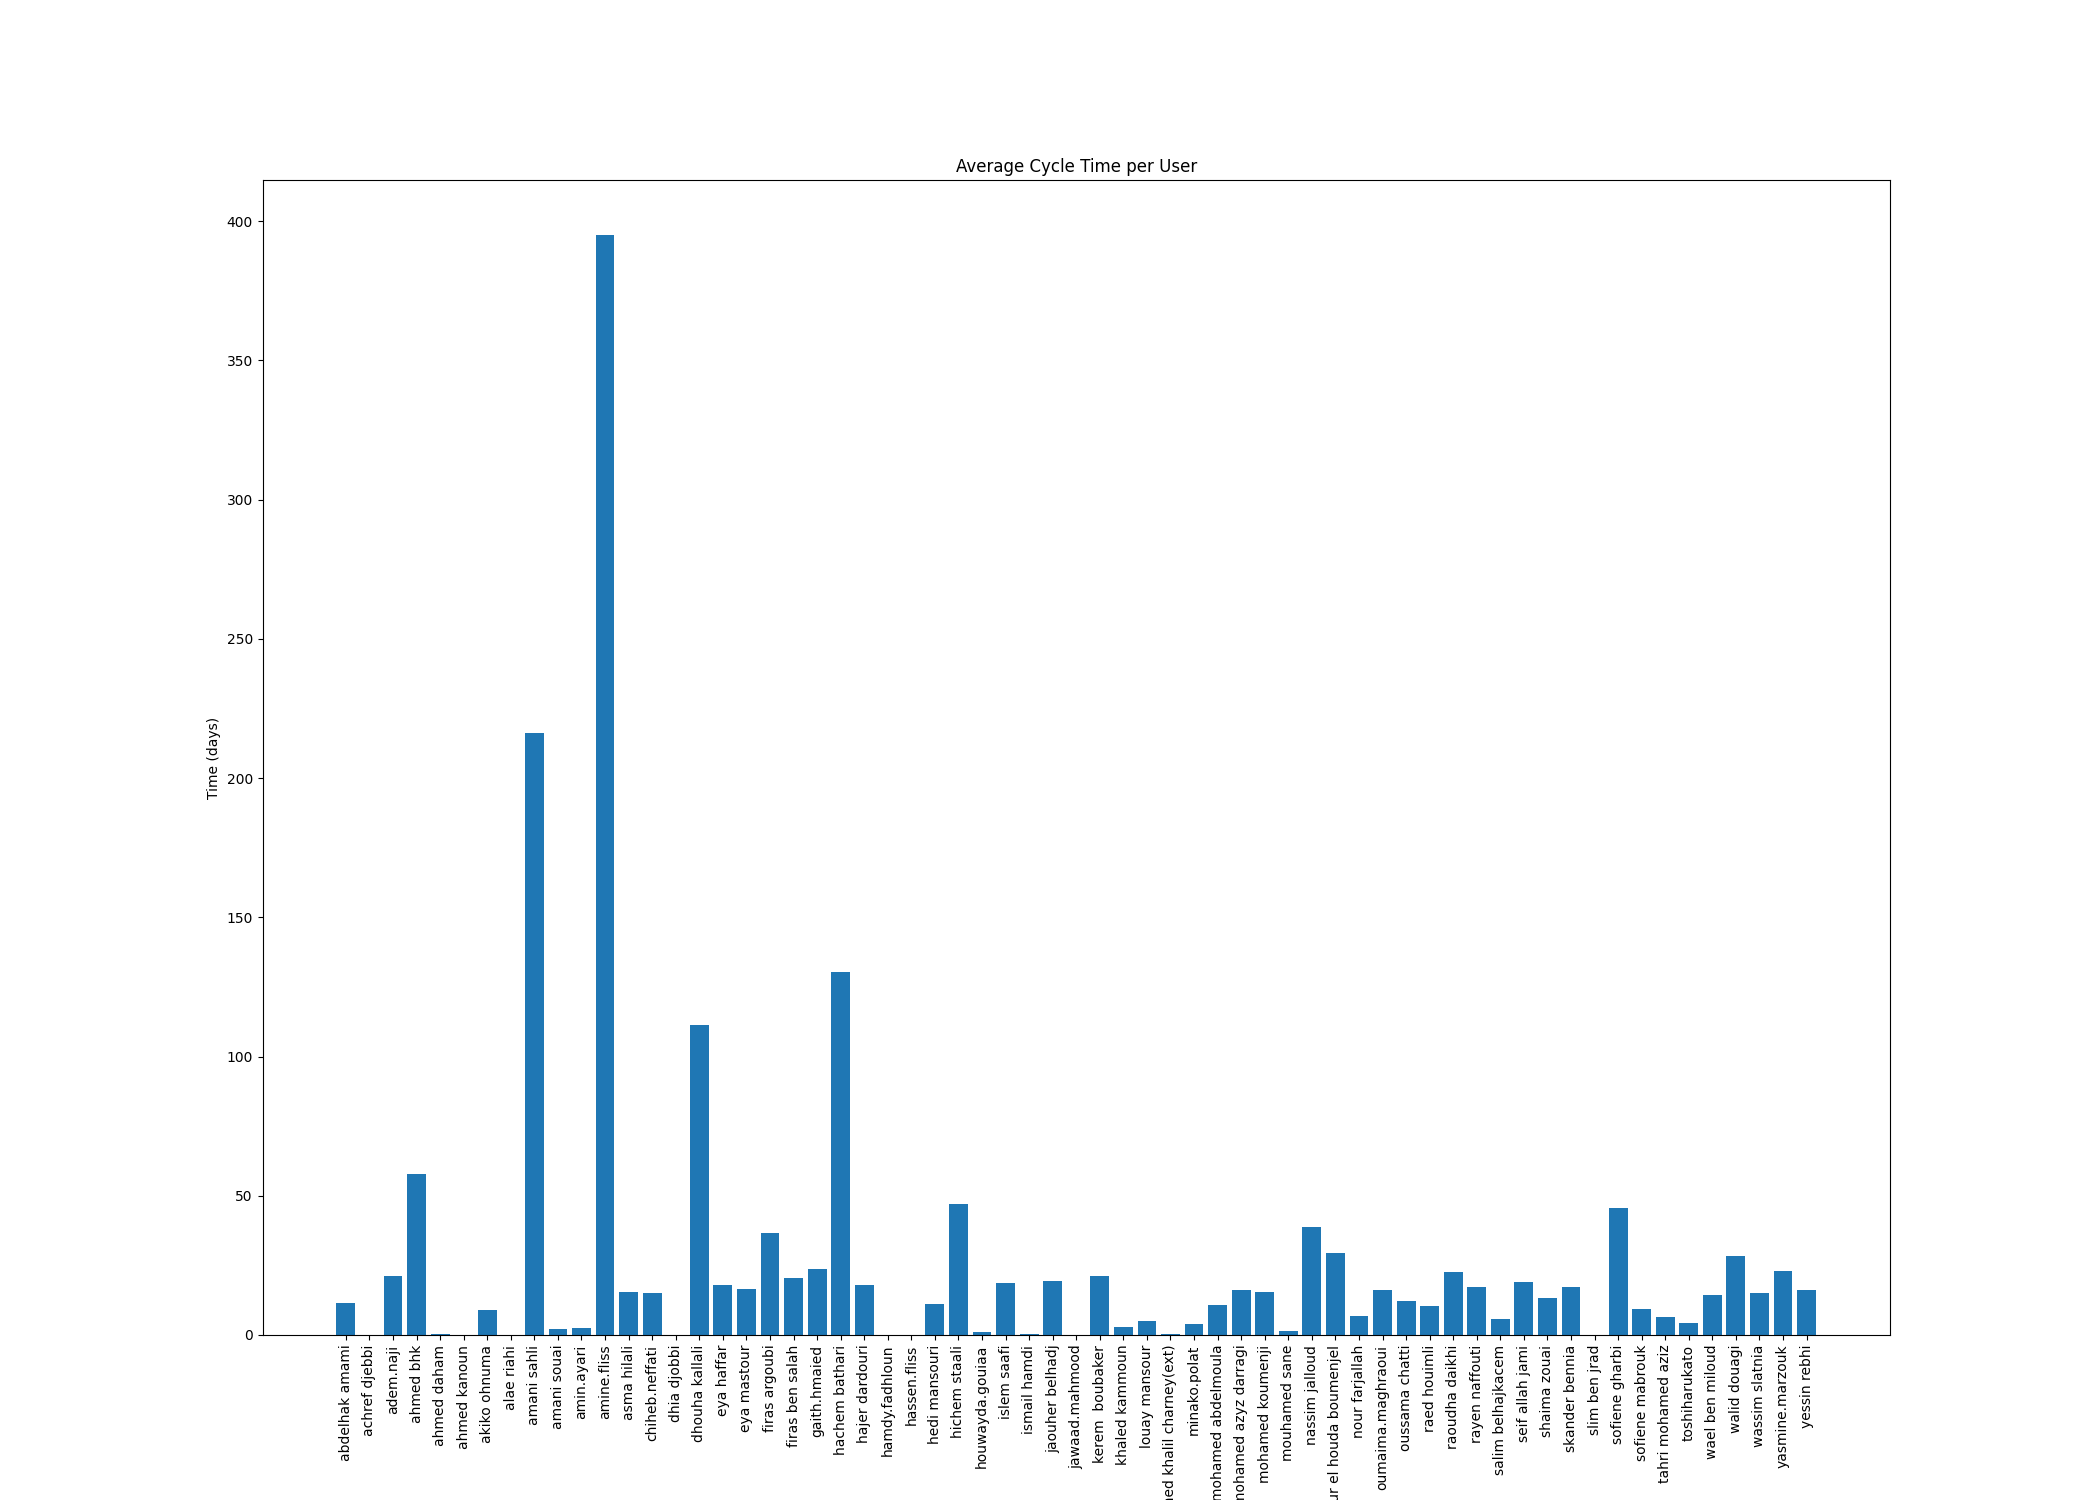
\includegraphics[width=1\linewidth,height=8cm]{img/captures/averge_cycle.png}
                \caption{Graphe de temps moyen de résolution des tickets par utilisateur}
                \label{fig:cycle}
            \end{figure}
            \par D'une part, on a constaté que cette corrélation a un impact important sur le temps de résolution des tickets et à la qualité du travail de ce collaborateur, de tel façon que: plus un utilisateur a de tickets assignés, plus son temps de résolution moyen est long, ce qui suggère une charge de travail plus lourde.
            \par D'une autre part, ces modelés aussi ont relevé une autre corrélation entre le nombres des tickets assignées à chaque collaborateur et sa productivité. En effet, les utilisateurs qui ont un grand nombre de tickets assignés sont également les plus productifs, ce qui pourrait indiquer une efficacité dans la gestion de leur charge de travail qui est représenté par la figure \textbf{\ref{fig:count}}. 
             \begin{figure}[H]
                \centering
                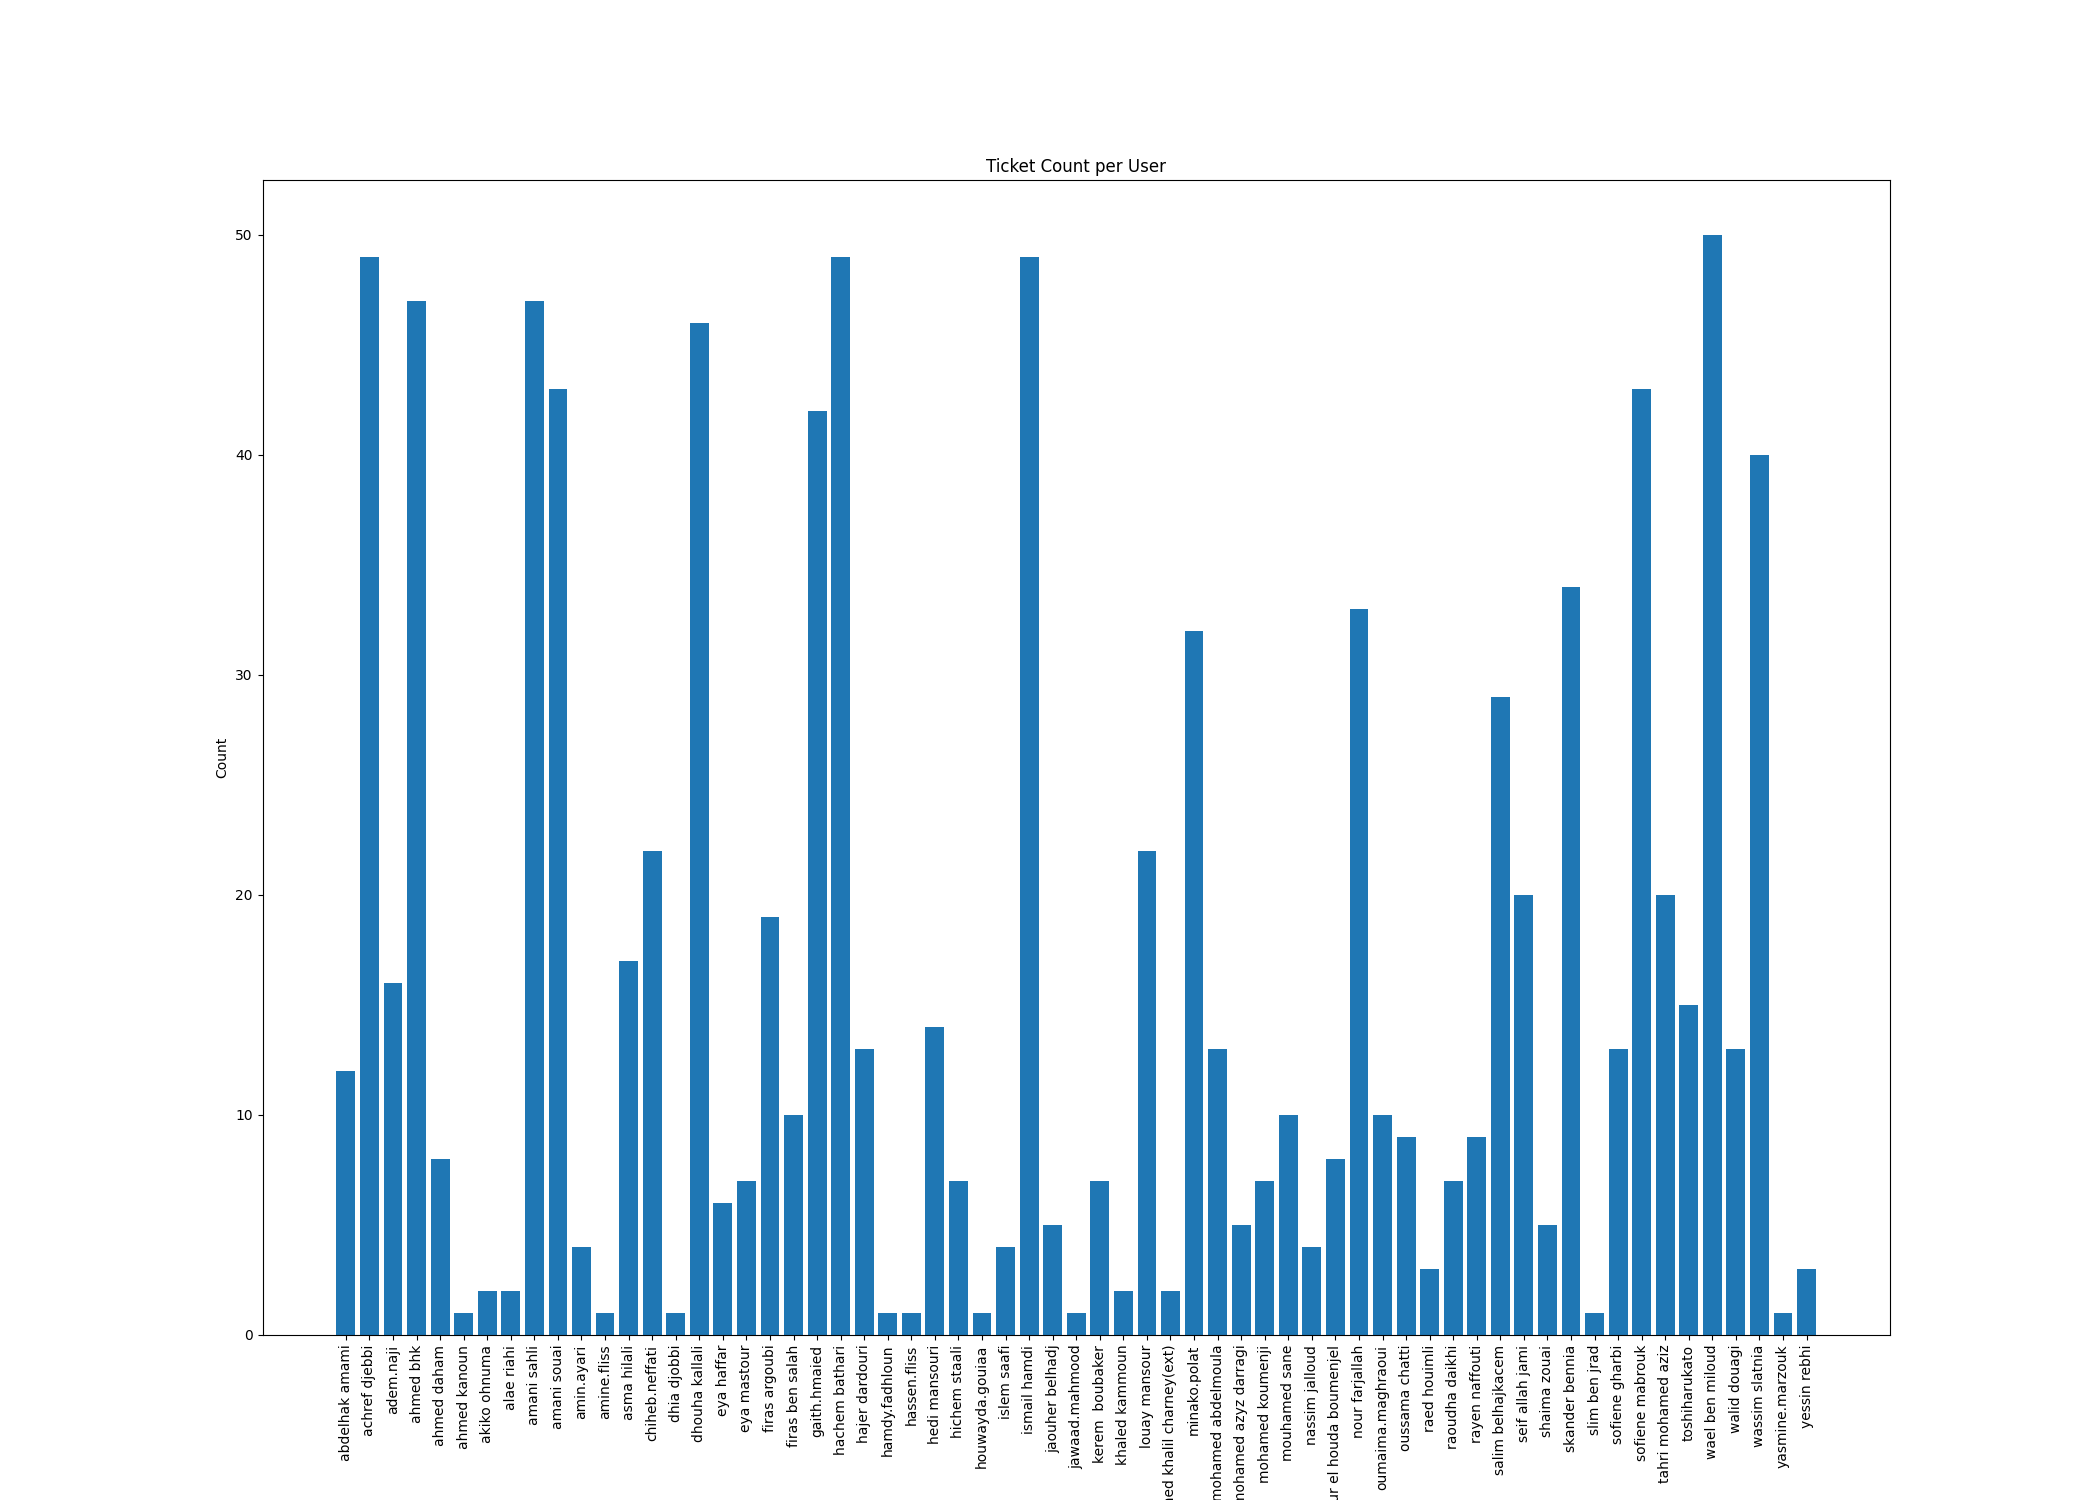
\includegraphics[width=1\linewidth,height=8cm]{img/captures/tickets_count.png}
                \caption{Graphe de productivité par rapport au nombre de tickets assignés à chaque collaborateur}
                \label{fig:count}
            \end{figure}
            \item \textbf{Identification des tendances et des axes d'amélioration:} l'analyse des données a mis en lumière des tendances dans les performances de l'équipe. Nous avons identifié les domaines où l'équipe excellait, ainsi que ceux qui nécessitaient des améliorations. Ces constats ont été partagés avec l'équipe pour orienter les décisions et les actions futures.
            \par la figure \textbf{\ref{fig:KPI}} suivante montre une partie de la fonction qui aide à étudier les KPI de l'équipe dont on va utilisé ultérieurement dans le dashbord. 
             \begin{figure}[H]
                \centering
                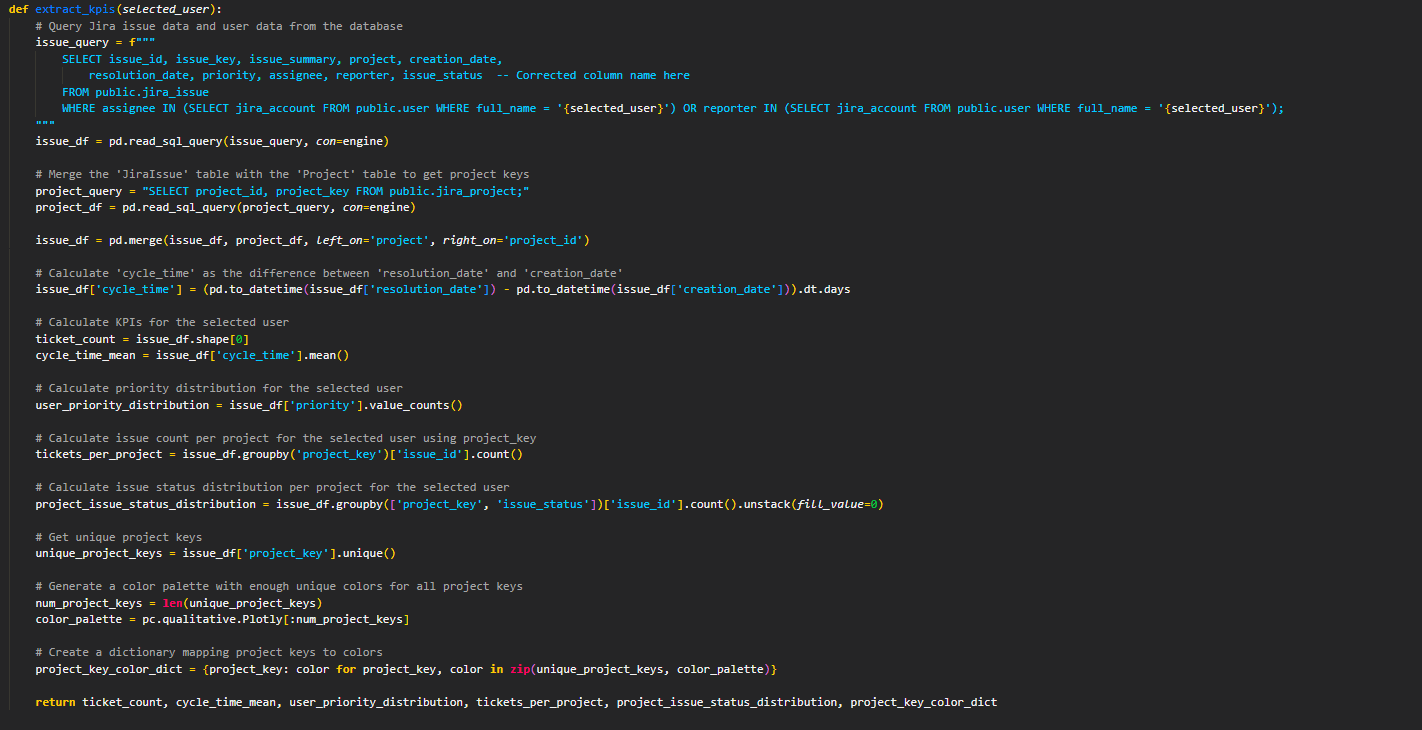
\includegraphics[width=1\linewidth]{img/captures/extractKPI.png}
                \caption{Fonction de l'extraction des KPI des collaborateurs}
                \label{fig:KPI}
            \end{figure}
        \end{itemize}
        \par L'étape d'analyse des données s'est révélée cruciale pour transformer des données brutes en connaissances exploitables. Elle a joué un rôle central dans la prise de décisions éclairées visant à améliorer les performances de l'équipe et à atteindre les objectifs du projet.
        \subsection{Visualisation des données}
        \par Suite à l'analyse des données et à l'identification de tendances significatives, il devenait impératif de présenter les résultats de manière claire et concise à l'équipe Avaxia. Cette phase consistait à élaborer des rapports et des visualisations dans le but d'informer et de guider les membres de l'équipe dans leurs actions. Voici comment nous avons abordé cette dernière étape :
        \begin{itemize}
            \item \textbf{Élaboration de tableaux de bord:} nous avons utilisé l'outil Streamlit pour créer des tableaux de bord interactifs mettant en évidence les principales conclusions de notre analyse. Ces tableaux de bord offraient une vue synthétique des performances de l'équipe, en mettant en avant les tendances clés, et permettaient une exploration interactive des données.
            \item \textbf{Utilisation de visualisations graphiques: }les visualisations graphiques ont revêtu une importance capitale dans la présentation des résultats. Nous avons employé divers types de graphiques, de diagrammes et de représentations visuelles pour illustrer les données. Cela incluait des graphiques de tendance, des histogrammes, des diagrammes circulaires, ainsi que d'autres formes graphiques pertinentes.
           
        
            \item \textbf{Présentation aux membres de l'équipe:} nous avons organisé une réunion de présentation pour communiquer les résultats à l'équipe Avaxia. Lors de cette réunion, nous avons mis en évidence les conclusions majeures, répondu aux questions et entamé des discussions sur les implications pour l'équipe.
            \item \textbf{Feedback et échanges:} après la présentation, nous avons encouragé les membres de l'équipe à partager leurs retours, poser des questions et discuter des prochaines étapes. Cette interaction était cruciale pour garantir une bonne compréhension des résultats et la prise de décisions éclairées.
        \end{itemize}
        \newpage
         \par La figure \textbf{\ref{fig:cap0}}, représente des captures d'écrans extraites du page tableau de bord principale de notre solution dont chaqune d'eux affiches des représenataions graphiques des différents analyses globales d'Avaxia.

        \begin{figure}[H]

            \begin{minipage}{1\linewidth}
            \centering
           % \subfloat{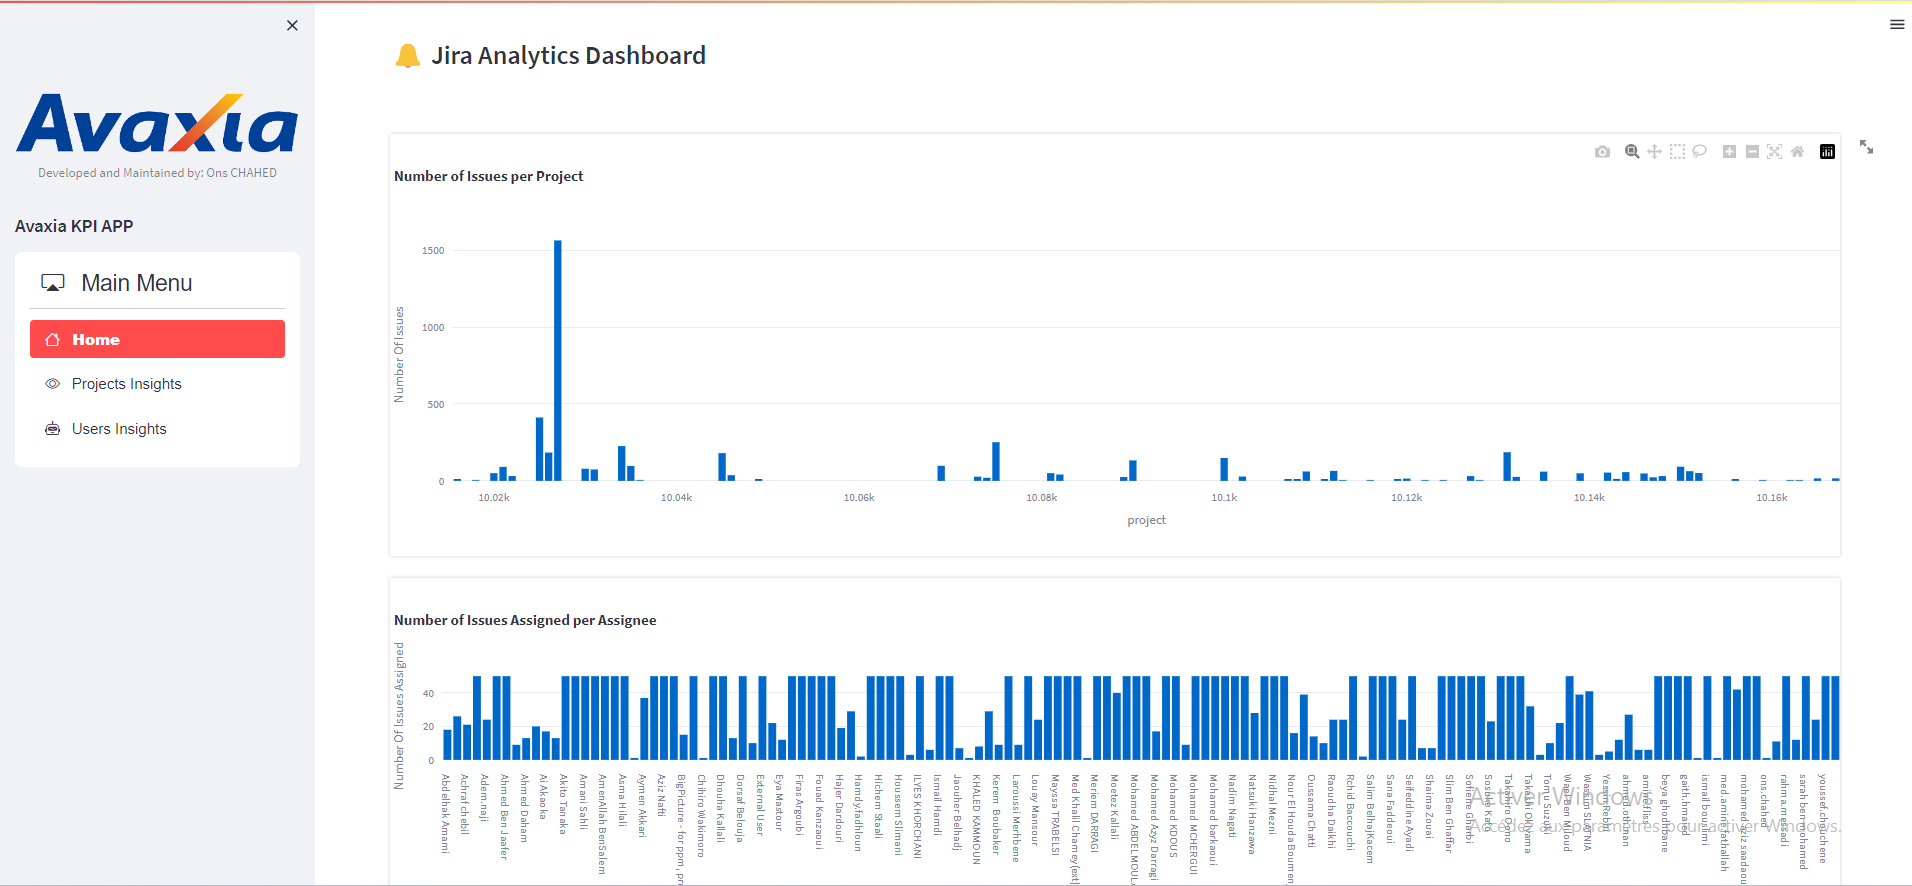
\includegraphics[width=1\linewidth , height=6.75cm]{img//captures/cap0.png}}\hspace{0.5cm}
           % \subfloat{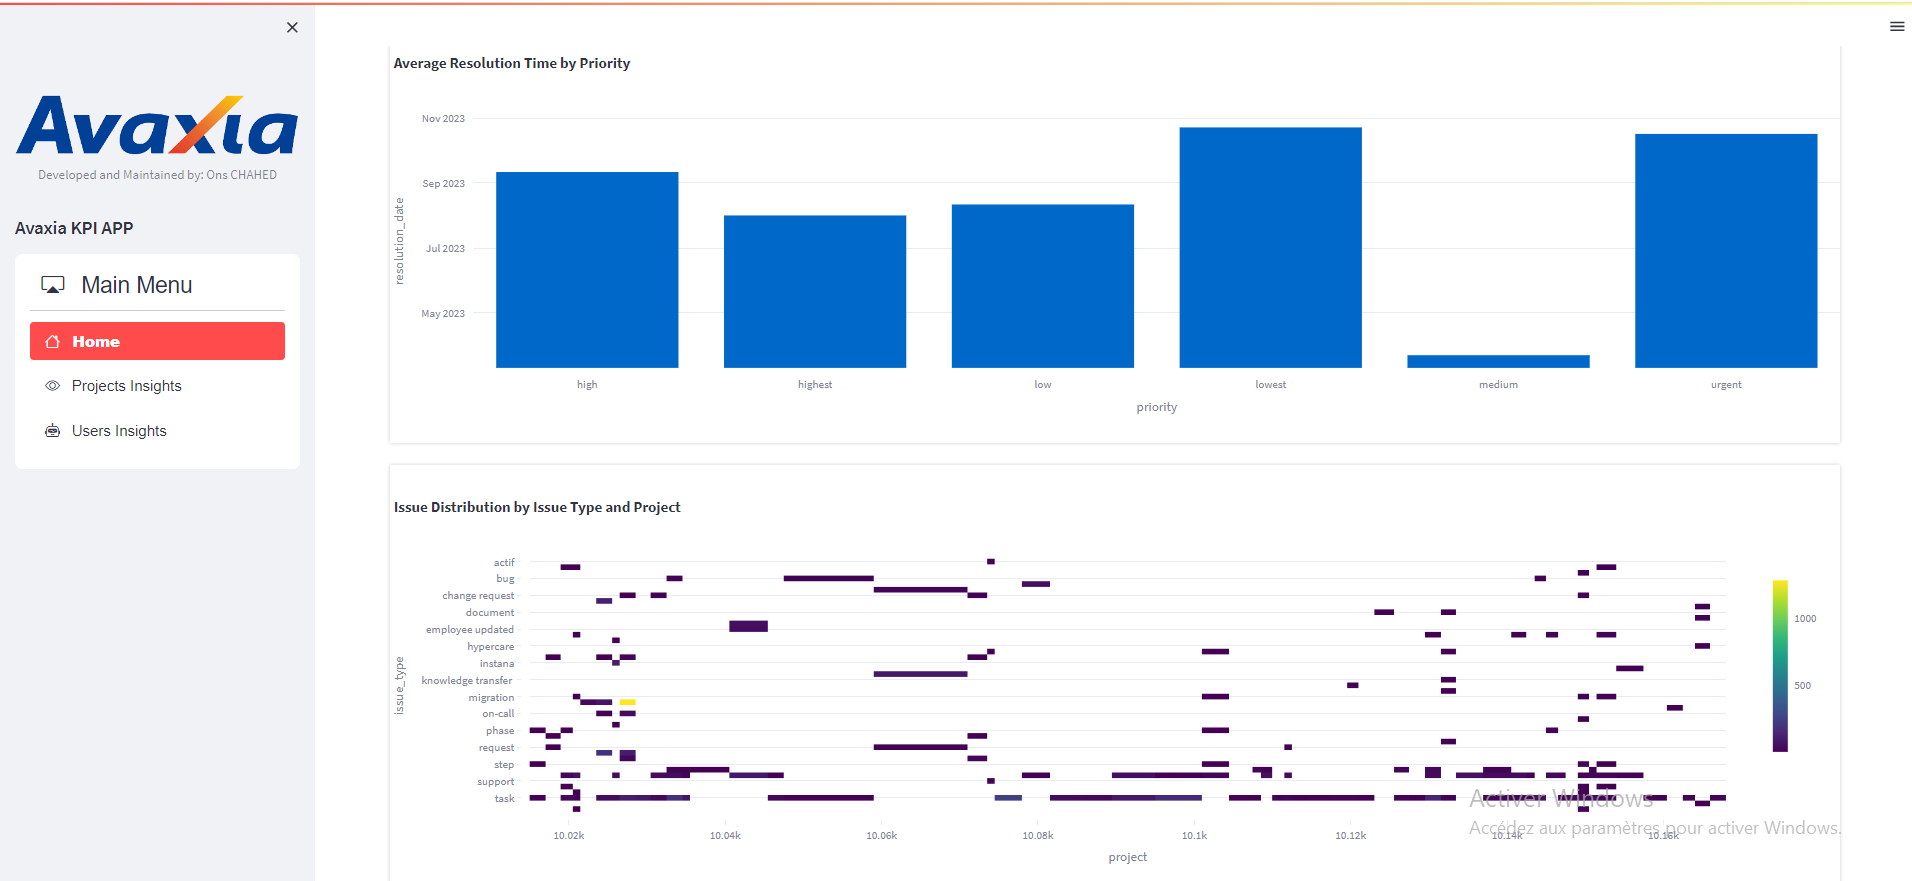
\includegraphics[width=1\linewidth, height=6.75cm]{img//captures/cap1.png}}\hspace{0.5cm}
            %\subfloat{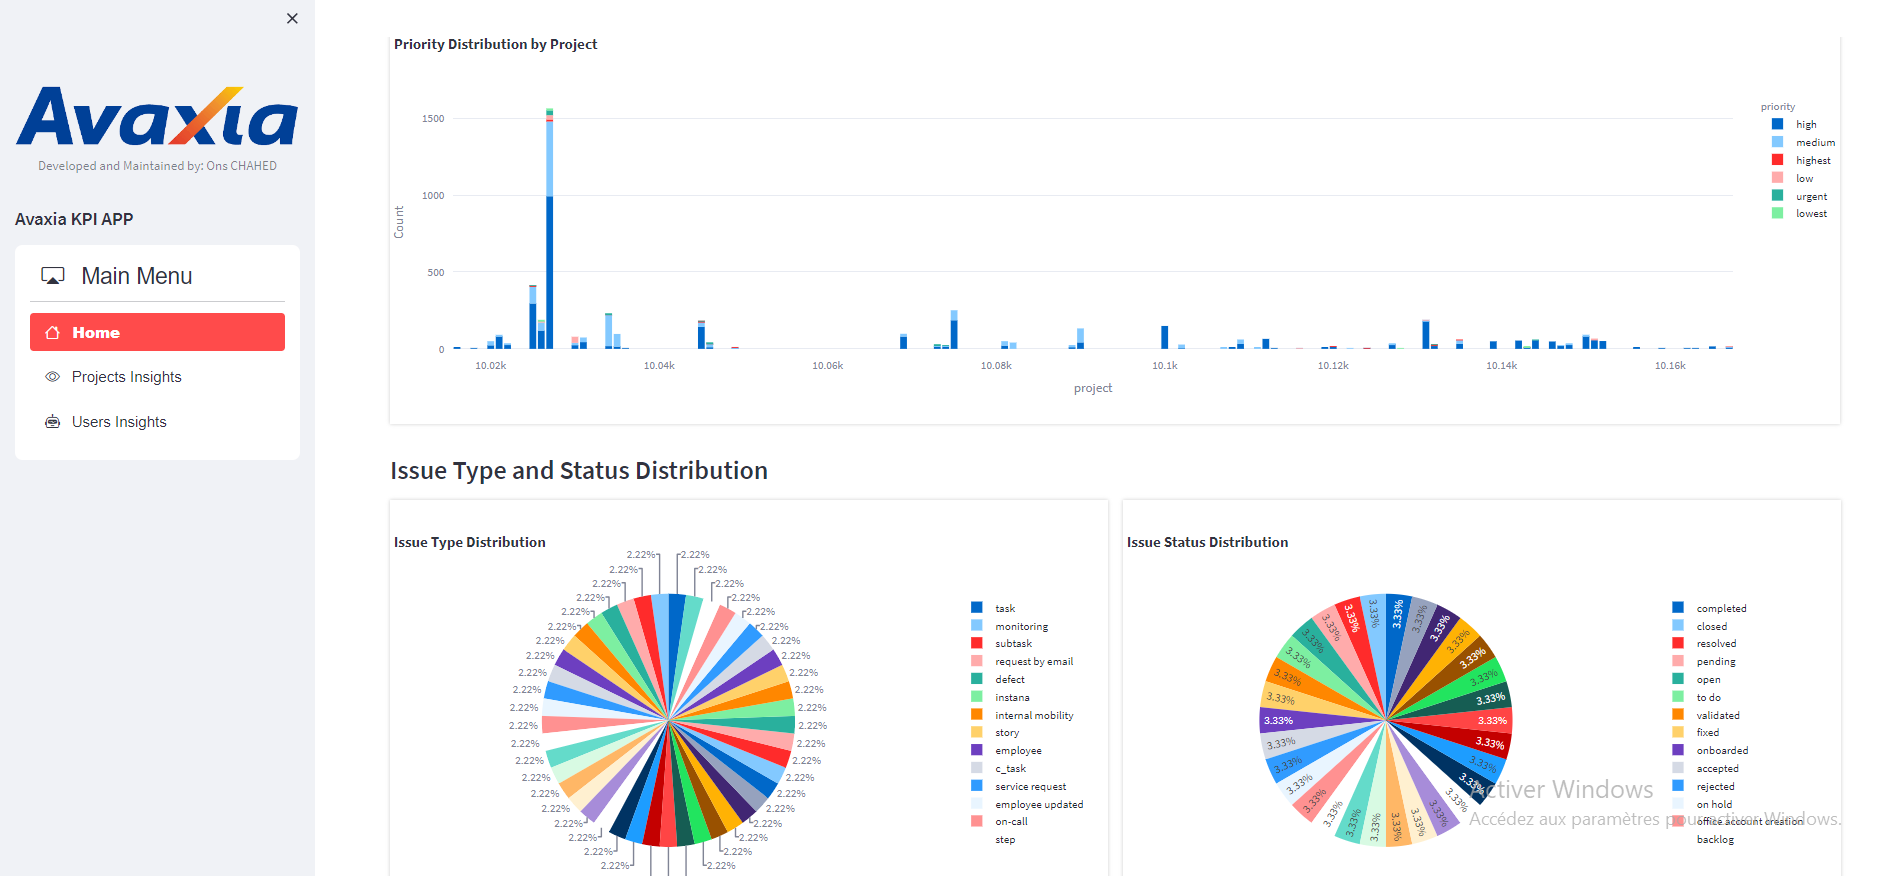
\includegraphics[width=1\linewidth , height=6.75cm]{img//captures/cap3.png}}

            \caption{Interface d'acceuil du tableau de bord}
            \label{fig:cap0}
             \end{minipage}\hfill 
        \end{figure}
         \par Les figures \textbf{\ref{fig:cap1}} représente des captures d'écrans extraites du page tableau de bord du section \textbf{<<Projects Insghits>>} dont on a choisi le projet \textbf{<<AeroSimEx Project>>}, son tableau \textbf{<<jira AeroSimEx Board>>} et le \textbf{<<sprint 13>>} pour afficher les différents statistiques de ces tickets.

        \begin{figure}[H]

            \begin{minipage}{1\linewidth}
            \centering
            %\subfloat{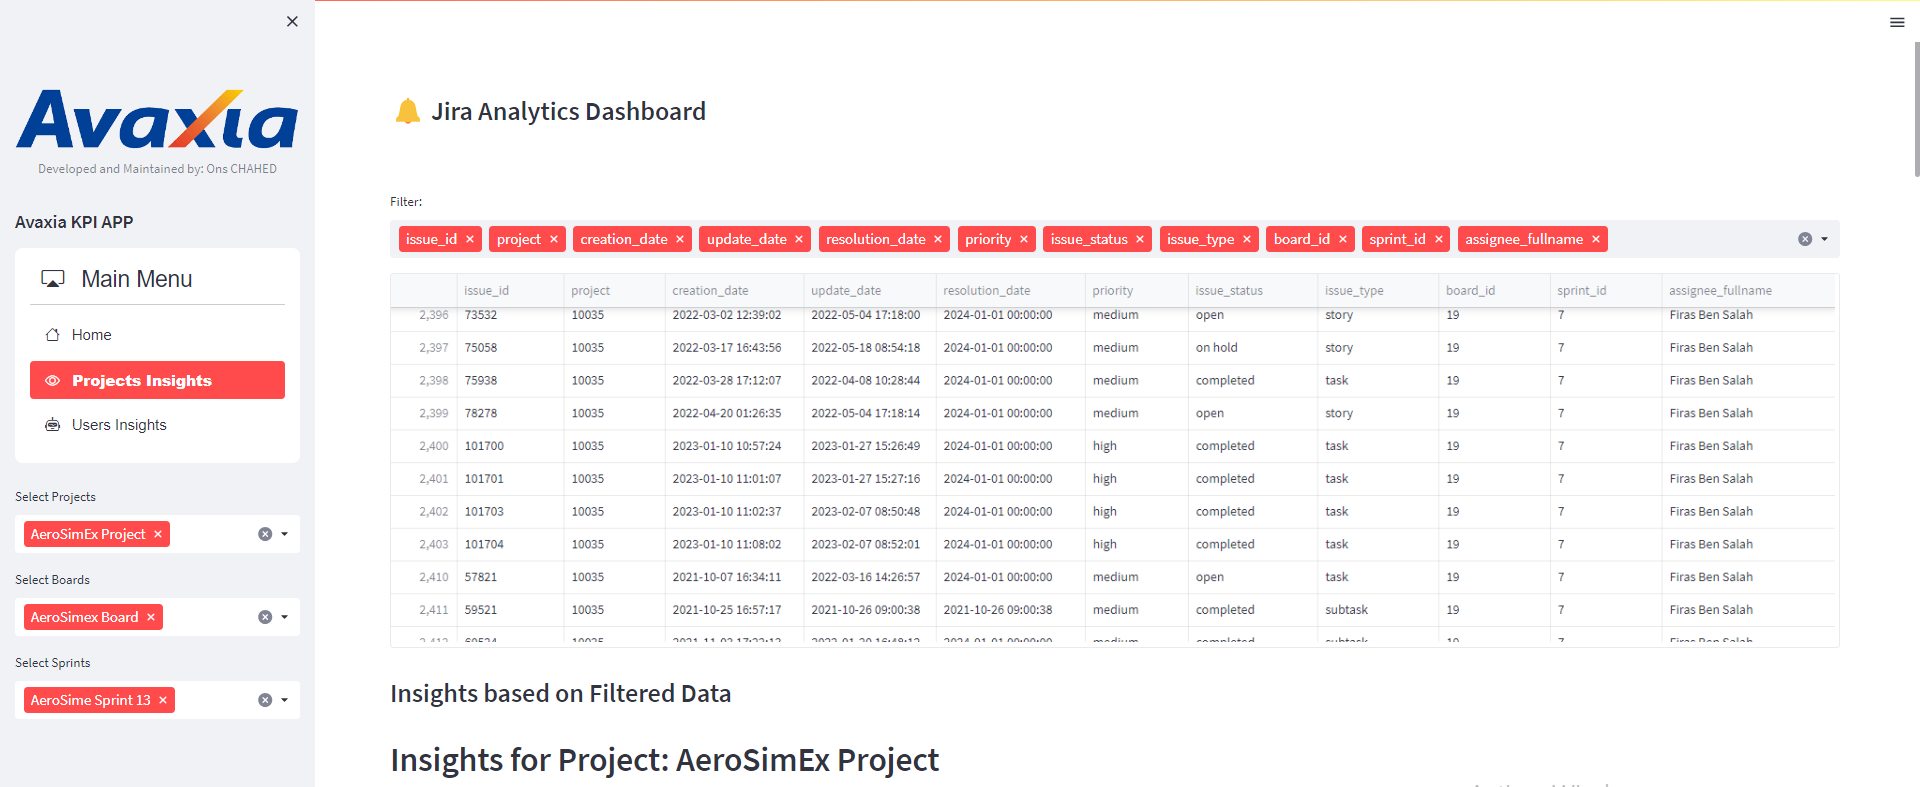
\includegraphics[width=1\linewidth , height=5cm]{img//captures/aero1.png}}\hspace{0.5cm}
           % \subfloat{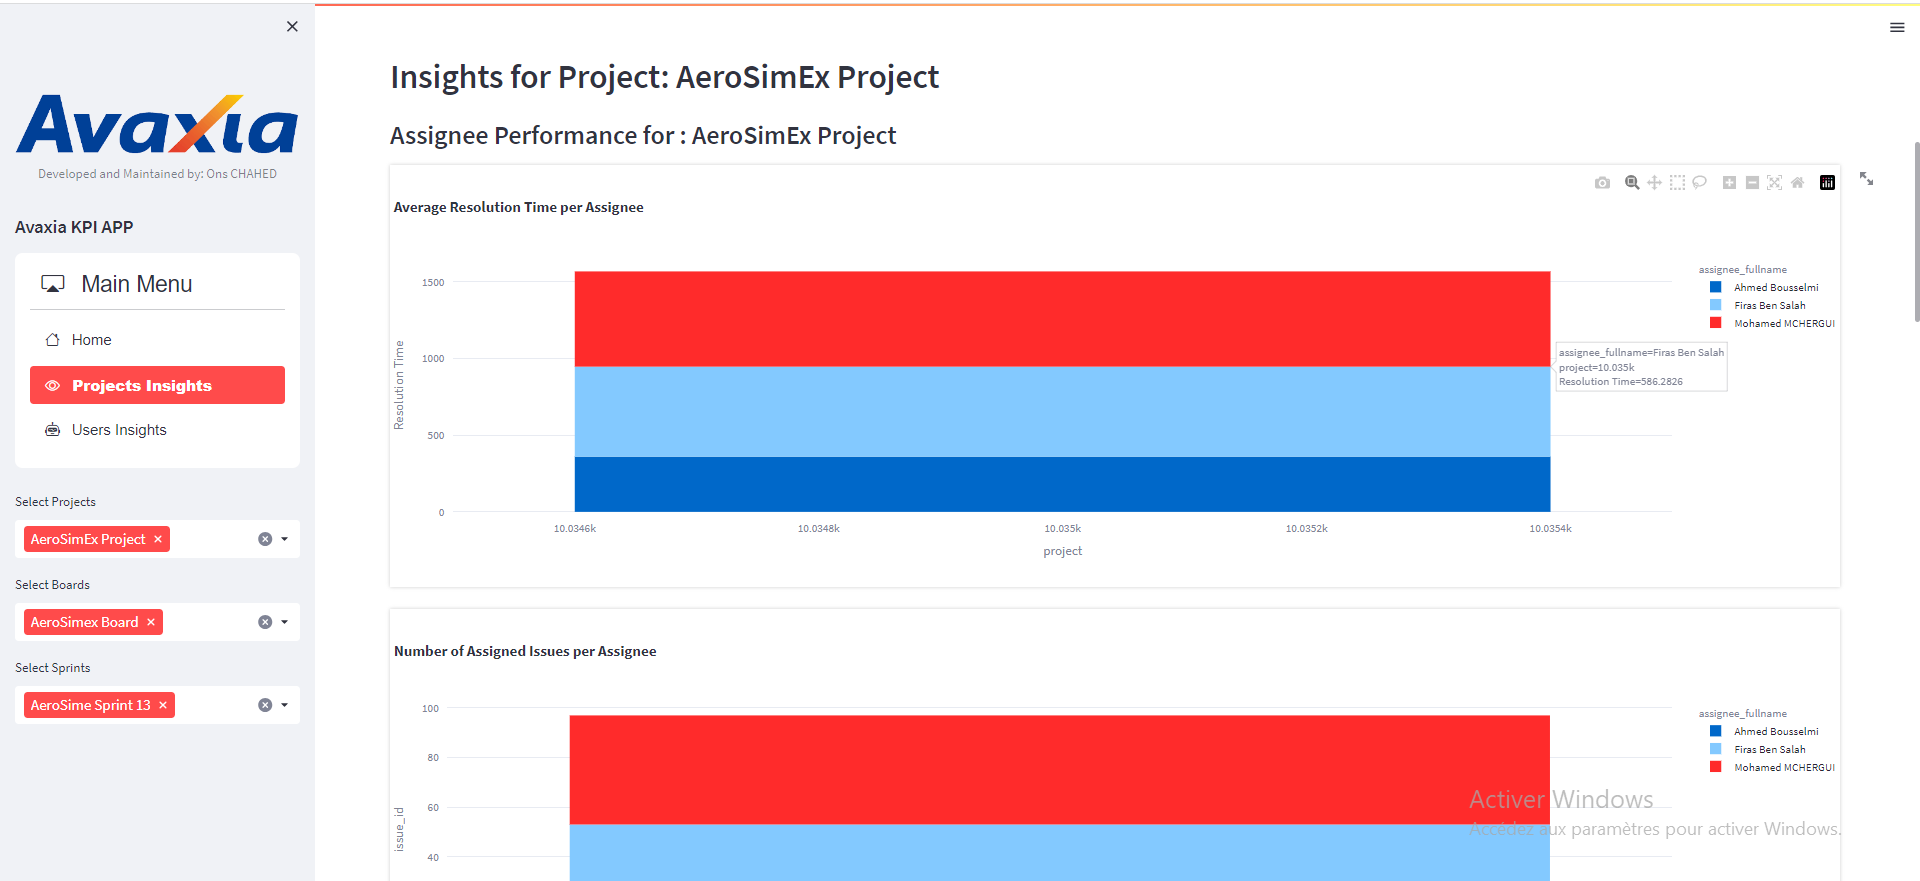
\includegraphics[width=1\linewidth, height=5cm]{img//captures/aero2.png}}\hspace{0.5cm}
            %\subfloat{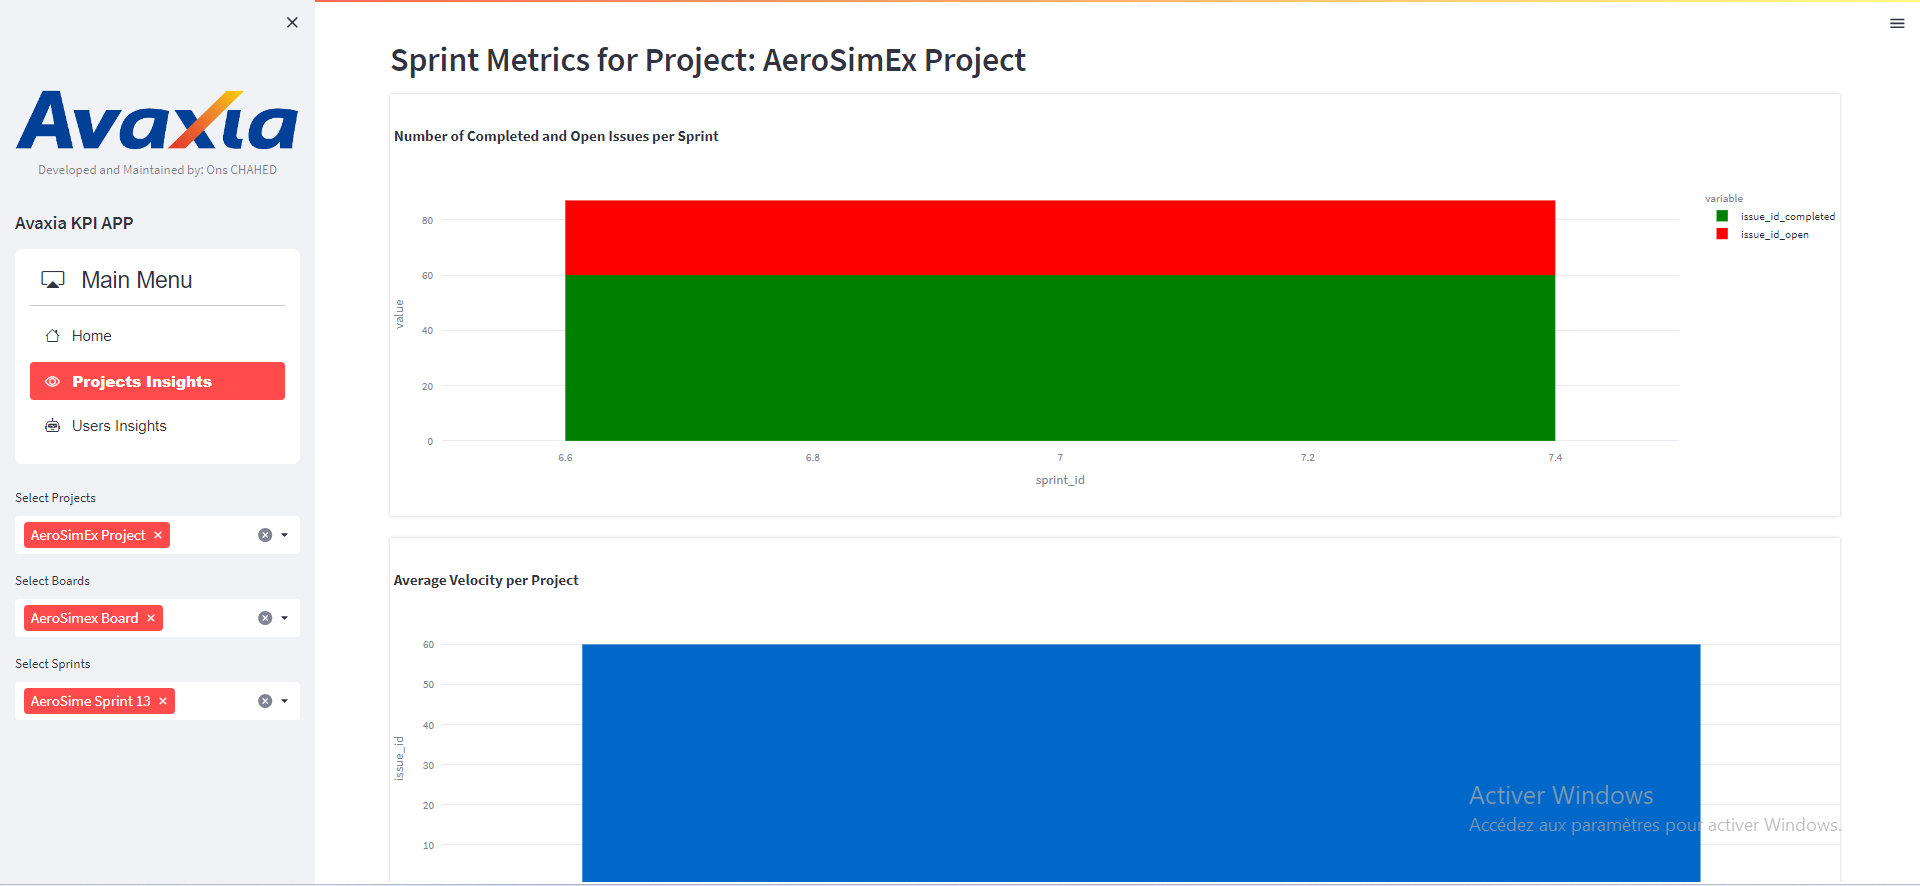
\includegraphics[width=1\linewidth , height=5cm]{img//captures/aero3.png}}\hspace{0.5cm}
            %\subfloat{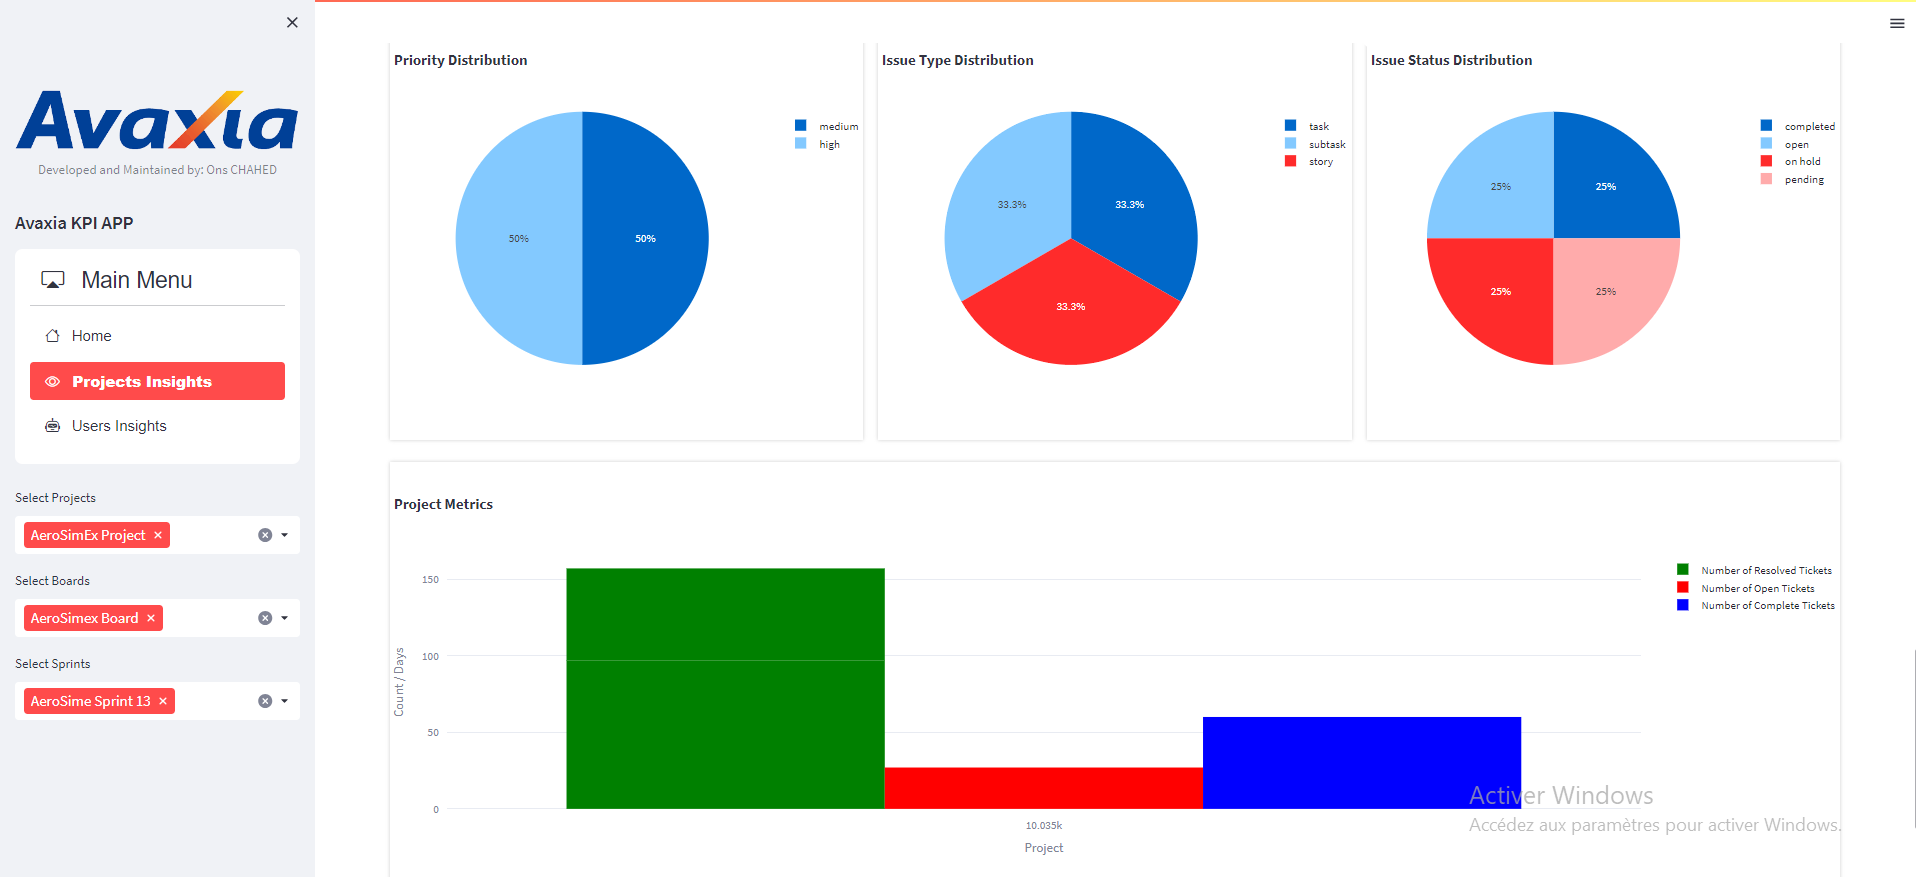
\includegraphics[width=1\linewidth , height=5cm]{img//captures/aero4.png}}

            \caption{Interface des statistiques du projet <<AeroSimEx Project>>}
       \label{fig:cap1}
             \end{minipage}\hfill 
        \end{figure}
         \par La figure \textbf{\ref{fig:cap2}} représente des captures d'écrans extraites du page tableau de bord du section \textbf{<<Users Insghits>>} dont on a choisi l'utilisateur \textbf{<<Nassim JALLOUD>>} pour afficher ces différents statistiques.

        \begin{figure}[H]

            \begin{minipage}{1\linewidth}
            \centering
           % \subfloat{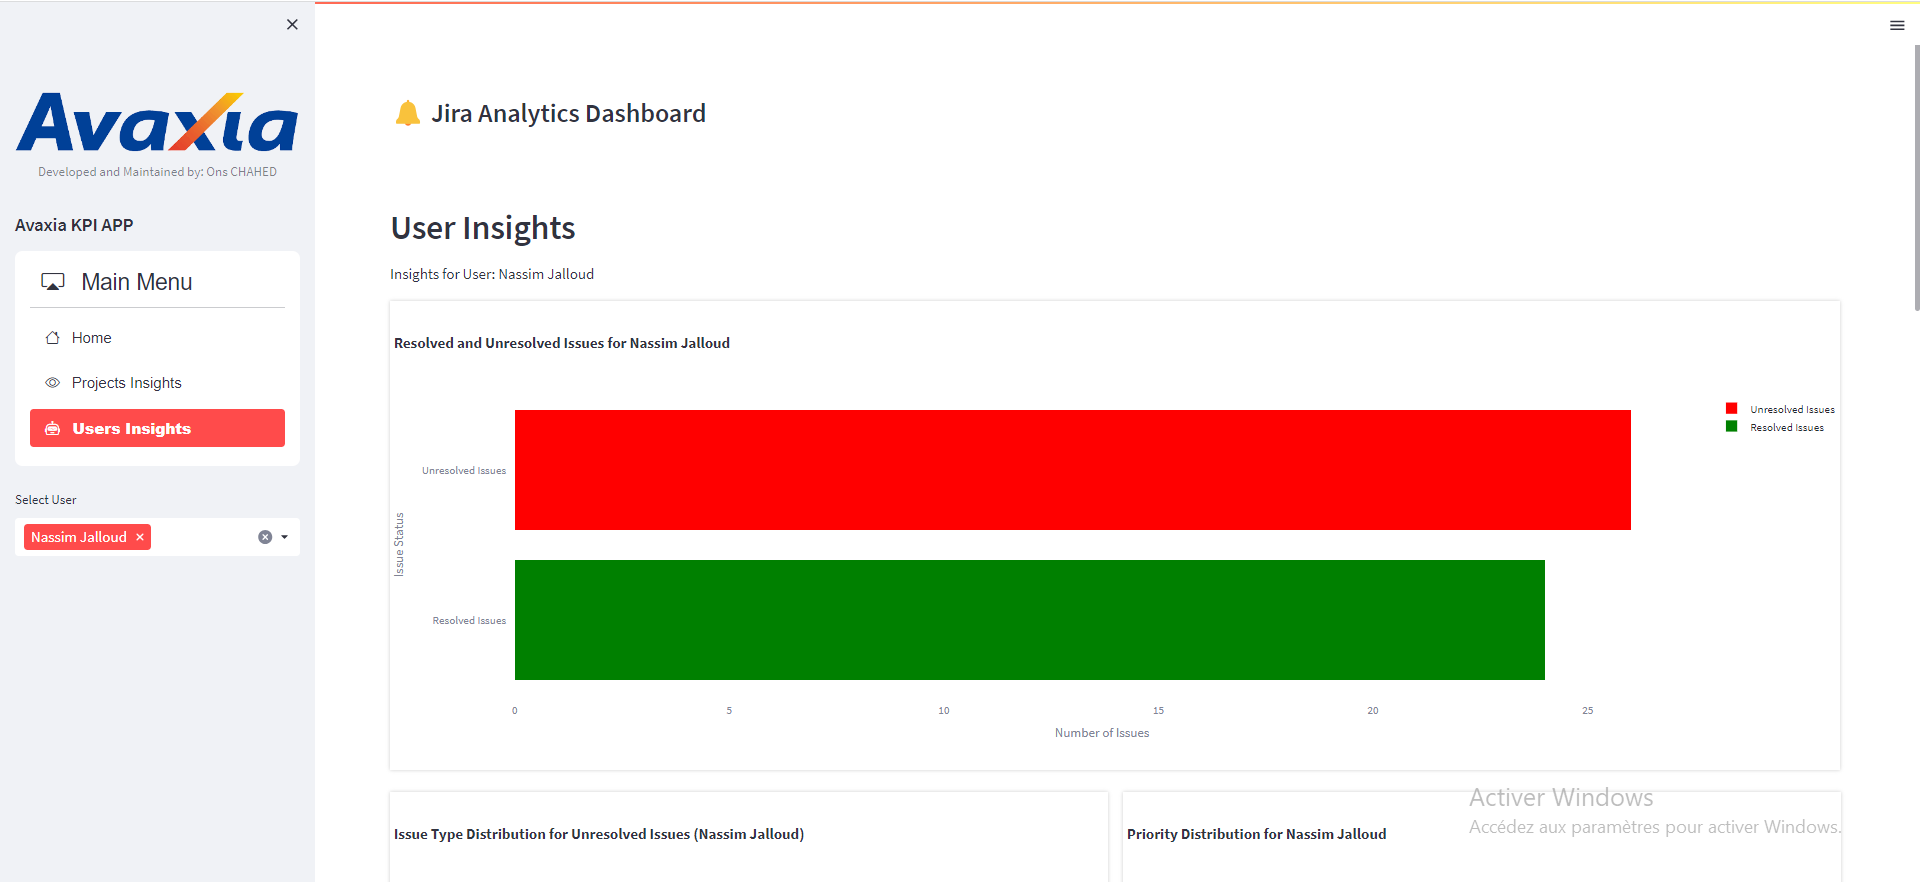
\includegraphics[width=1\linewidth , height=6.75cm]{img//captures/user1.png}}\hspace{0.5cm}
            %\subfloat{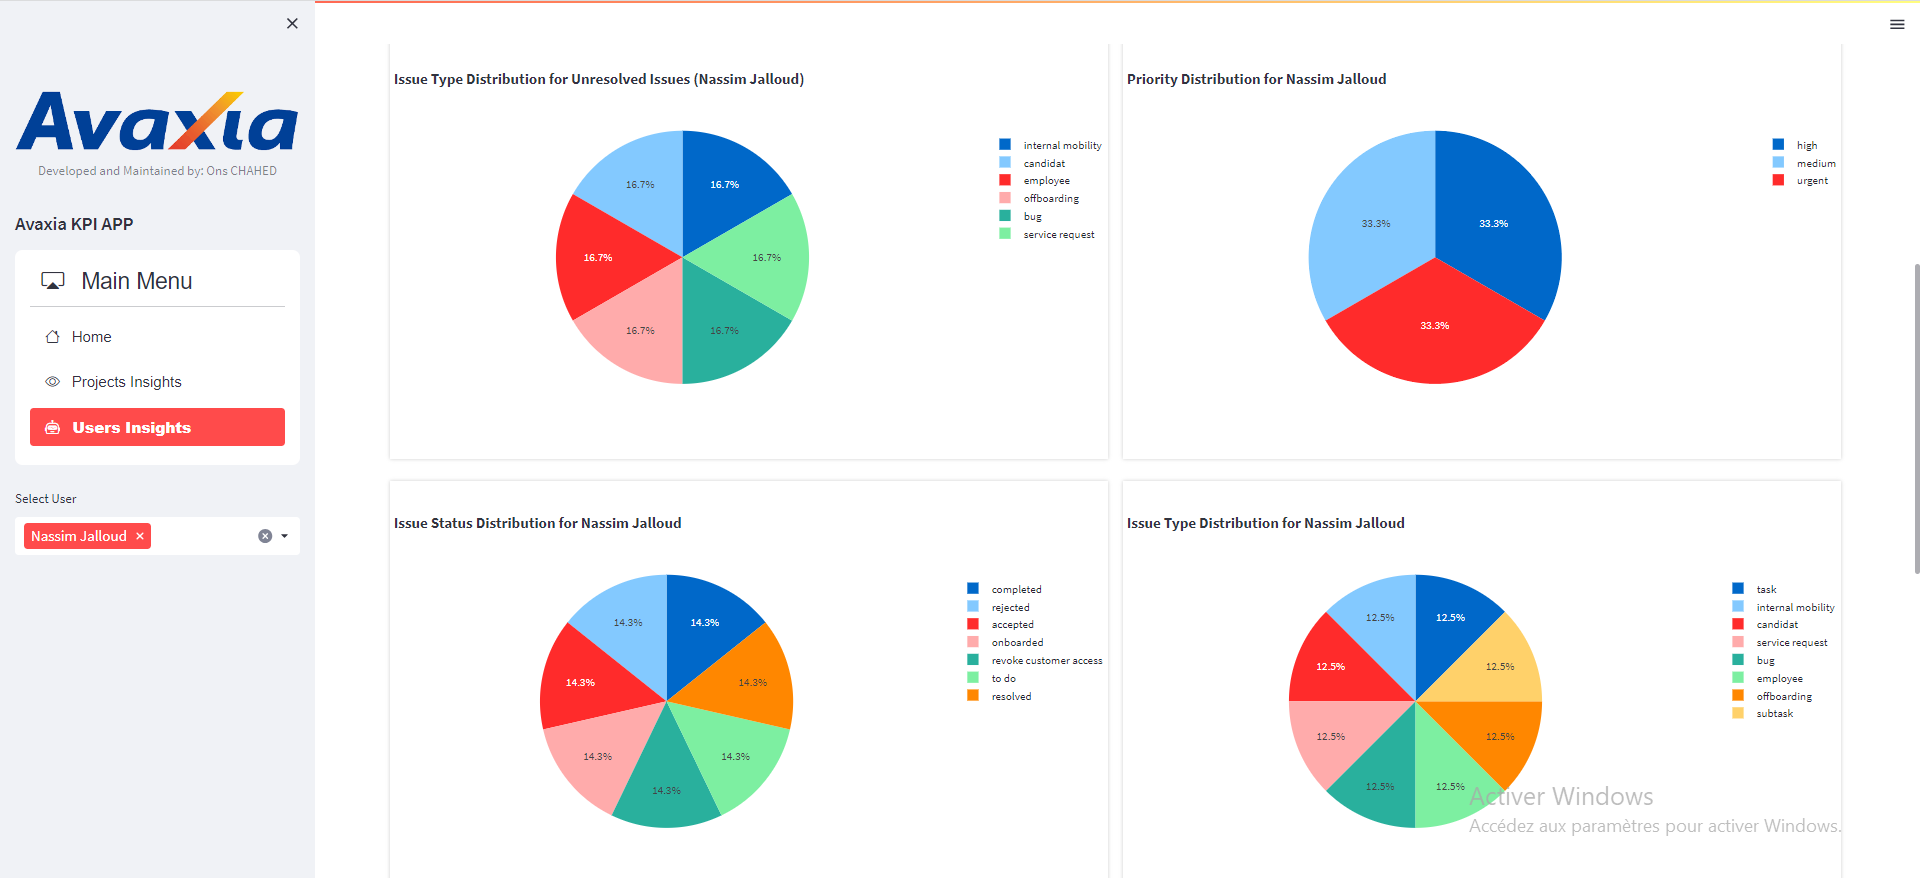
\includegraphics[width=1\linewidth, height=6.75cm]{img//captures/user2.png}}\hspace{0.5cm}
            %\subfloat{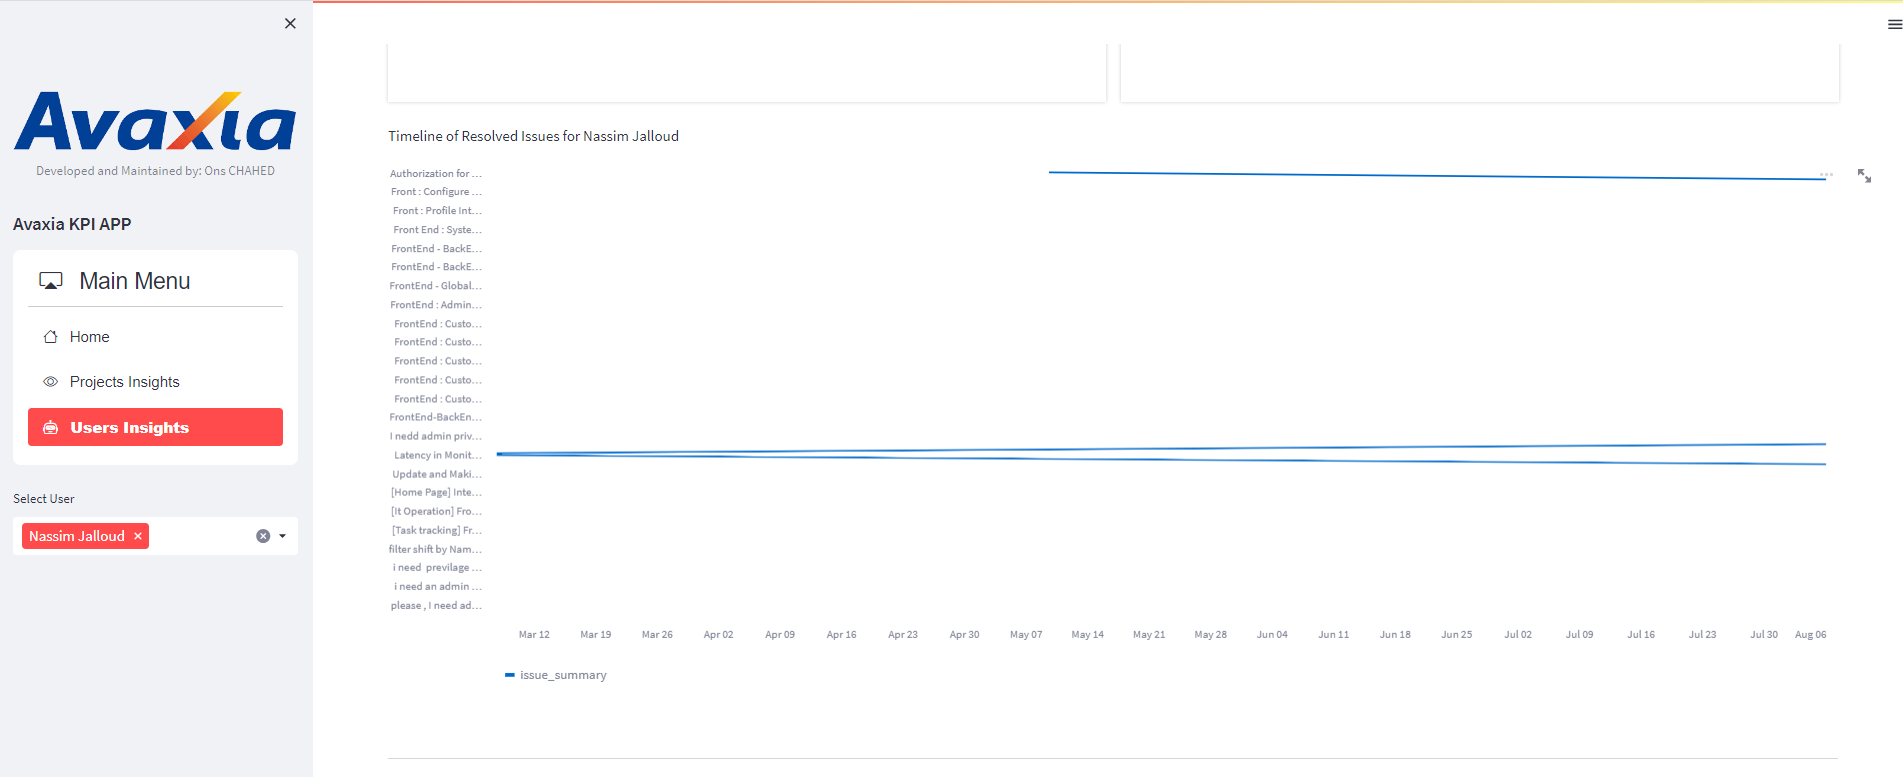
\includegraphics[width=1\linewidth , height=6.75cm]{img//captures/user3.png}}

            \caption{Interface des statistiques de l'utilisateur <<Nassim JALLOUD>>}
            \label{fig:cap2}
             \end{minipage}\hfill 
        \end{figure}
        \par L'étape de communication des constatations était essentielle pour s'assurer que les informations et les recommandations découlant de l'analyse des données étaient pertinentes et actionnables. Elle a fourni à l'équipe Avaxia une vue nette de ses performances et des domaines nécessitant des améliorations, contribuant ainsi à la réalisation des objectifs du projet.
        
\section*{Conclusion}
\addcontentsline{toc}{section}{Conclusion }
    Ce chapitre résume le travail accompli pour donner forme à notre projet. Les choix techniques et le workflow nous ont fourni un cadre solide pour concrétiser notre vision. Chaque étape de ce processus s'avère cruciale pour l'atteinte de nos objectifs.
    \par Dans la conclusion générale à venir, nous réunirons l'ensemble de notre travail et soulignerons les perspectives pour l'avenir.